\documentclass[8pt]{beamer}
%\usepackage[T1]{fontenc}% pour la sortie
\usepackage[utf8]{inputenc}
\usepackage{amsmath}
\usepackage{mathrsfs}
\usepackage{amssymb}
\usepackage{xcolor}
\usepackage{fancyhdr}
\usepackage{color}
\usepackage{bm}
\usepackage{cases}
\usepackage{comment}
\usepackage{tabto}
\usepackage{changepage}

\usepackage{pict2e}
\usepackage{pgfplots}

\usepackage{graphicx}
\usepackage{kbordermatrix} 
\usepackage{listings} 
\usepackage{tikz}
\usetikzlibrary{tikzmark}
\usetikzlibrary {graphs,shapes.geometric}
\usetikzlibrary{arrows.meta}
\usetikzlibrary{graphdrawing}
\usegdlibrary{circular}
\tikzset{
mystyle/.style={
  circle,
  inner sep=1pt,
  text width=12.4mm,
  align=center,
  draw=black,
  fill=white
  }
}

\lstset
{
    language=[LaTeX]TeX,
    breaklines=true,
    basicstyle=\tt\normalsize,
    keywordstyle=\color{blue},
    identifierstyle=\color{magenta},
    frame = single,
    numbers=left,
	numberstyle=\tiny \bf \color{blue},
	stepnumber=1,	
	numbersep=10pt,
	firstnumber=1,
	numberfirstline=true
}

\lstdefinestyle{python}{
basicstyle=\ttm\footnotesize,
morekeywords={self},              % Add keywords here
keywordstyle=\ttb\color{deepblue},
emph={MyClass,__init__},          % Custom highlighting
emphstyle=\ttb\color{deepred},    % Custom highlighting style
stringstyle=\color{deepgreen},
frame=tb,                         % Any extra options here
showstringspaces=false
}

\lstdefinestyle{asp}{
     basicstyle=\tt\footnotesize,
}

\lstdefinestyle{aspwide}{
     basicstyle=\tt\scriptsize,
}
 
\usepackage{multimedia}
\usepackage{sidecap}

\usepackage{hanging}
\usepackage{listings} 

\usepackage[natbib=true,style=authoryear,backend=bibtex,useprefix=true]{biblatex}
\addbibresource{bib.bib}

\setbeamertemplate{footnote}{%
  \hangpara{0.8em}{1}%
   \makebox[-0.4em][l]{\scriptsize\insertfootnotemark}\scriptsize\insertfootnotetext\par%
}

\newcommand*{\Scale}[2][4]{\scalebox{#1}{$\displaystyle{#2}$}}%
\newcommand{\ml}[1]{\textcolor{blue}{[\emph{ML} -- #1]}}

\lstset
{
    language=[LaTeX]TeX,
    breaklines=true,
    basicstyle=\tt\normalsize,
    keywordstyle=\color{blue},
    identifierstyle=\color{magenta},
    frame = single,
    numbers=left,
	numberstyle=\tiny \bf \color{blue},
	stepnumber=1,	
	numbersep=10pt,
	firstnumber=1,
	numberfirstline=true
}

\lstdefinestyle{asp}{
     basicstyle=\tt\footnotesize,
}

\DeclareMathOperator*{\logten}{log_{10}}

\usefonttheme[onlymath]{serif} %% Pour écrire les maths comme dans les documents latex classiques
\setbeamertemplate{navigation symbols}{} %% Pour enlever les symboles de navigation en bas à droite, peu utiles
  
% \usetheme{Warsaw}
\usetheme{Frankfurt}

\setbeamercolor{structure}{fg =blue!70}

\definecolor{mygreen}{rgb}{0, 0.6, 0}

\renewcommand{\kbldelim}{(}% Left delimiter
\renewcommand{\kbrdelim}{)}% Right delimiter

%%% Définition de l'en-tête de page
\setbeamercolor{headcolor1}{fg=white,bg=blue!70}
\setbeamercolor{headcolor2}{fg=white,bg=red!75}


\makeatletter

\def\insertnavigation#1{%
  \vbox{{%
    \usebeamerfont{section in head/foot}\usebeamercolor[fg]{section in head/foot}%
    \beamer@xpos=0\relax%
    \beamer@ypos=1\relax%
    \hbox to #1{\hskip.3cm\setbox\beamer@sectionbox=\hbox{\kern1sp}%
      \ht\beamer@sectionbox=1.875ex%
      \dp\beamer@sectionbox=0.75ex%
        \hskip.3cm%
        \global\beamer@section@min@dim\z@
        \dohead%
        \beamer@section@set@min@width
      \box\beamer@sectionbox\hfill\hskip.3cm}%
}}}%  
\setbeamertemplate{caption}[numbered]
\setbeamertemplate{headline}
{%
  \begin{beamercolorbox}[ht=2.25ex,dp=3.75ex]{headcolor1}
    \hskip-4ex\insertnavigation{\paperwidth}
  \end{beamercolorbox}%
}



%% Définition du pied de page
\setbeamercolor{footcolor}{fg=white,bg=blue!70}

\setbeamertemplate{footline}{
\leavevmode%
\hbox{\hspace*{-0.08cm}
\begin{beamercolorbox}[wd=.2\paperwidth,ht=2.7ex,dp=1ex,center]{footcolor}%
	\insertshortauthor
\end{beamercolorbox}%
\begin{beamercolorbox}[wd=.6\paperwidth,ht=2.7ex,dp=1ex,center]{footcolor}%
	\insertshorttitle
\end{beamercolorbox}%
\begin{beamercolorbox}[wd=.1\paperwidth,ht=2.7ex,dp=1ex,center]{footcolor}%
	\vspace{-0.07cm}
\includegraphics[width=0.3cm]{figures/bacteria.png}\hspace*{2em}
\includegraphics[width=0.3cm]{figures/bacteria_2.png}
%	\insertframenumber{} / \inserttotalframenumber\hspace*{2ex}
\end{beamercolorbox}}%
\begin{beamercolorbox}[wd=.1\paperwidth,ht=2.7ex,dp=1ex,right]{footcolor}%
	\insertframenumber{} / \inserttotalframenumber\hspace*{2ex}
\end{beamercolorbox}%
\vskip0pt%
}

\makeatother
\author[Maxime LECOMTE]{Présenté par Maxime LECOMTE \vspace{-0.5cm}}
\title[Hybrid approach for explainable metabolic modelling of microbial ecosystems']{Approche hybride de modélisation explicable du métabolisme des écosystèmes microbiens}
\subtitle{Hybrid approach for explainable metabolic modelling of microbial ecosystems'}
\date{\today}

\usetikzlibrary{shapes,backgrounds}


\begin{document}

\begin{frame}

\maketitle
\small
{\centering\itshape Membres du jury\par}
Président: SIMON Laurent\par\medskip

\begin{tabular}[t]{@{}l@{\hspace{3pt}}p{.35\textwidth}@{}}
Rapportrices: & BAROUKH Caroline\\
& COCAIGN-BOUSQUET Muriel
\end{tabular}%
\newline

\begin{tabular}[t]{@{}l@{\hspace{3pt}}p{.32\textwidth}@{}}
Examinateurs: 
& COTTRET Ludovic \\
& LAROCHE Béatrice \\
& MARKOV Gabriel \vfill
\end{tabular}%
\footnotesize
\begin{tabular}[t]{@{}l@{\hspace{4pt}}p{.4\textwidth}@{}}
Co-direction: & David SHERMAN et Hélène FALENTIN \\
Encadrement: & Clémence FRIOUX
\end{tabular}%


\includegraphics[height=0.55cm]{figures/logos/logo_EDMI.png}
\hfill

\includegraphics[height=0.55cm]{figures/logos/Logo-INRAE_Transparent.png}
\hfill

\includegraphics[height=0.55cm]{figures/logos/logo_inria.png}
\hfill

\includegraphics[height=0.55cm]{figures/logos/logo_LaBRI.png}

\end{frame}



%%%%%%%%%%%%%%%%%%%%%%%%%%%%%%%%%%%%%%%%%%%%%%%%%%%%%%%%%%%%%%%%%%%%%%%%%%%%%%%%%%%
\section{Motivation}

\begin{frame}
\frametitle{Why the study of microorganisms is relevant ?}
\begin{figure}[t]
\centering   
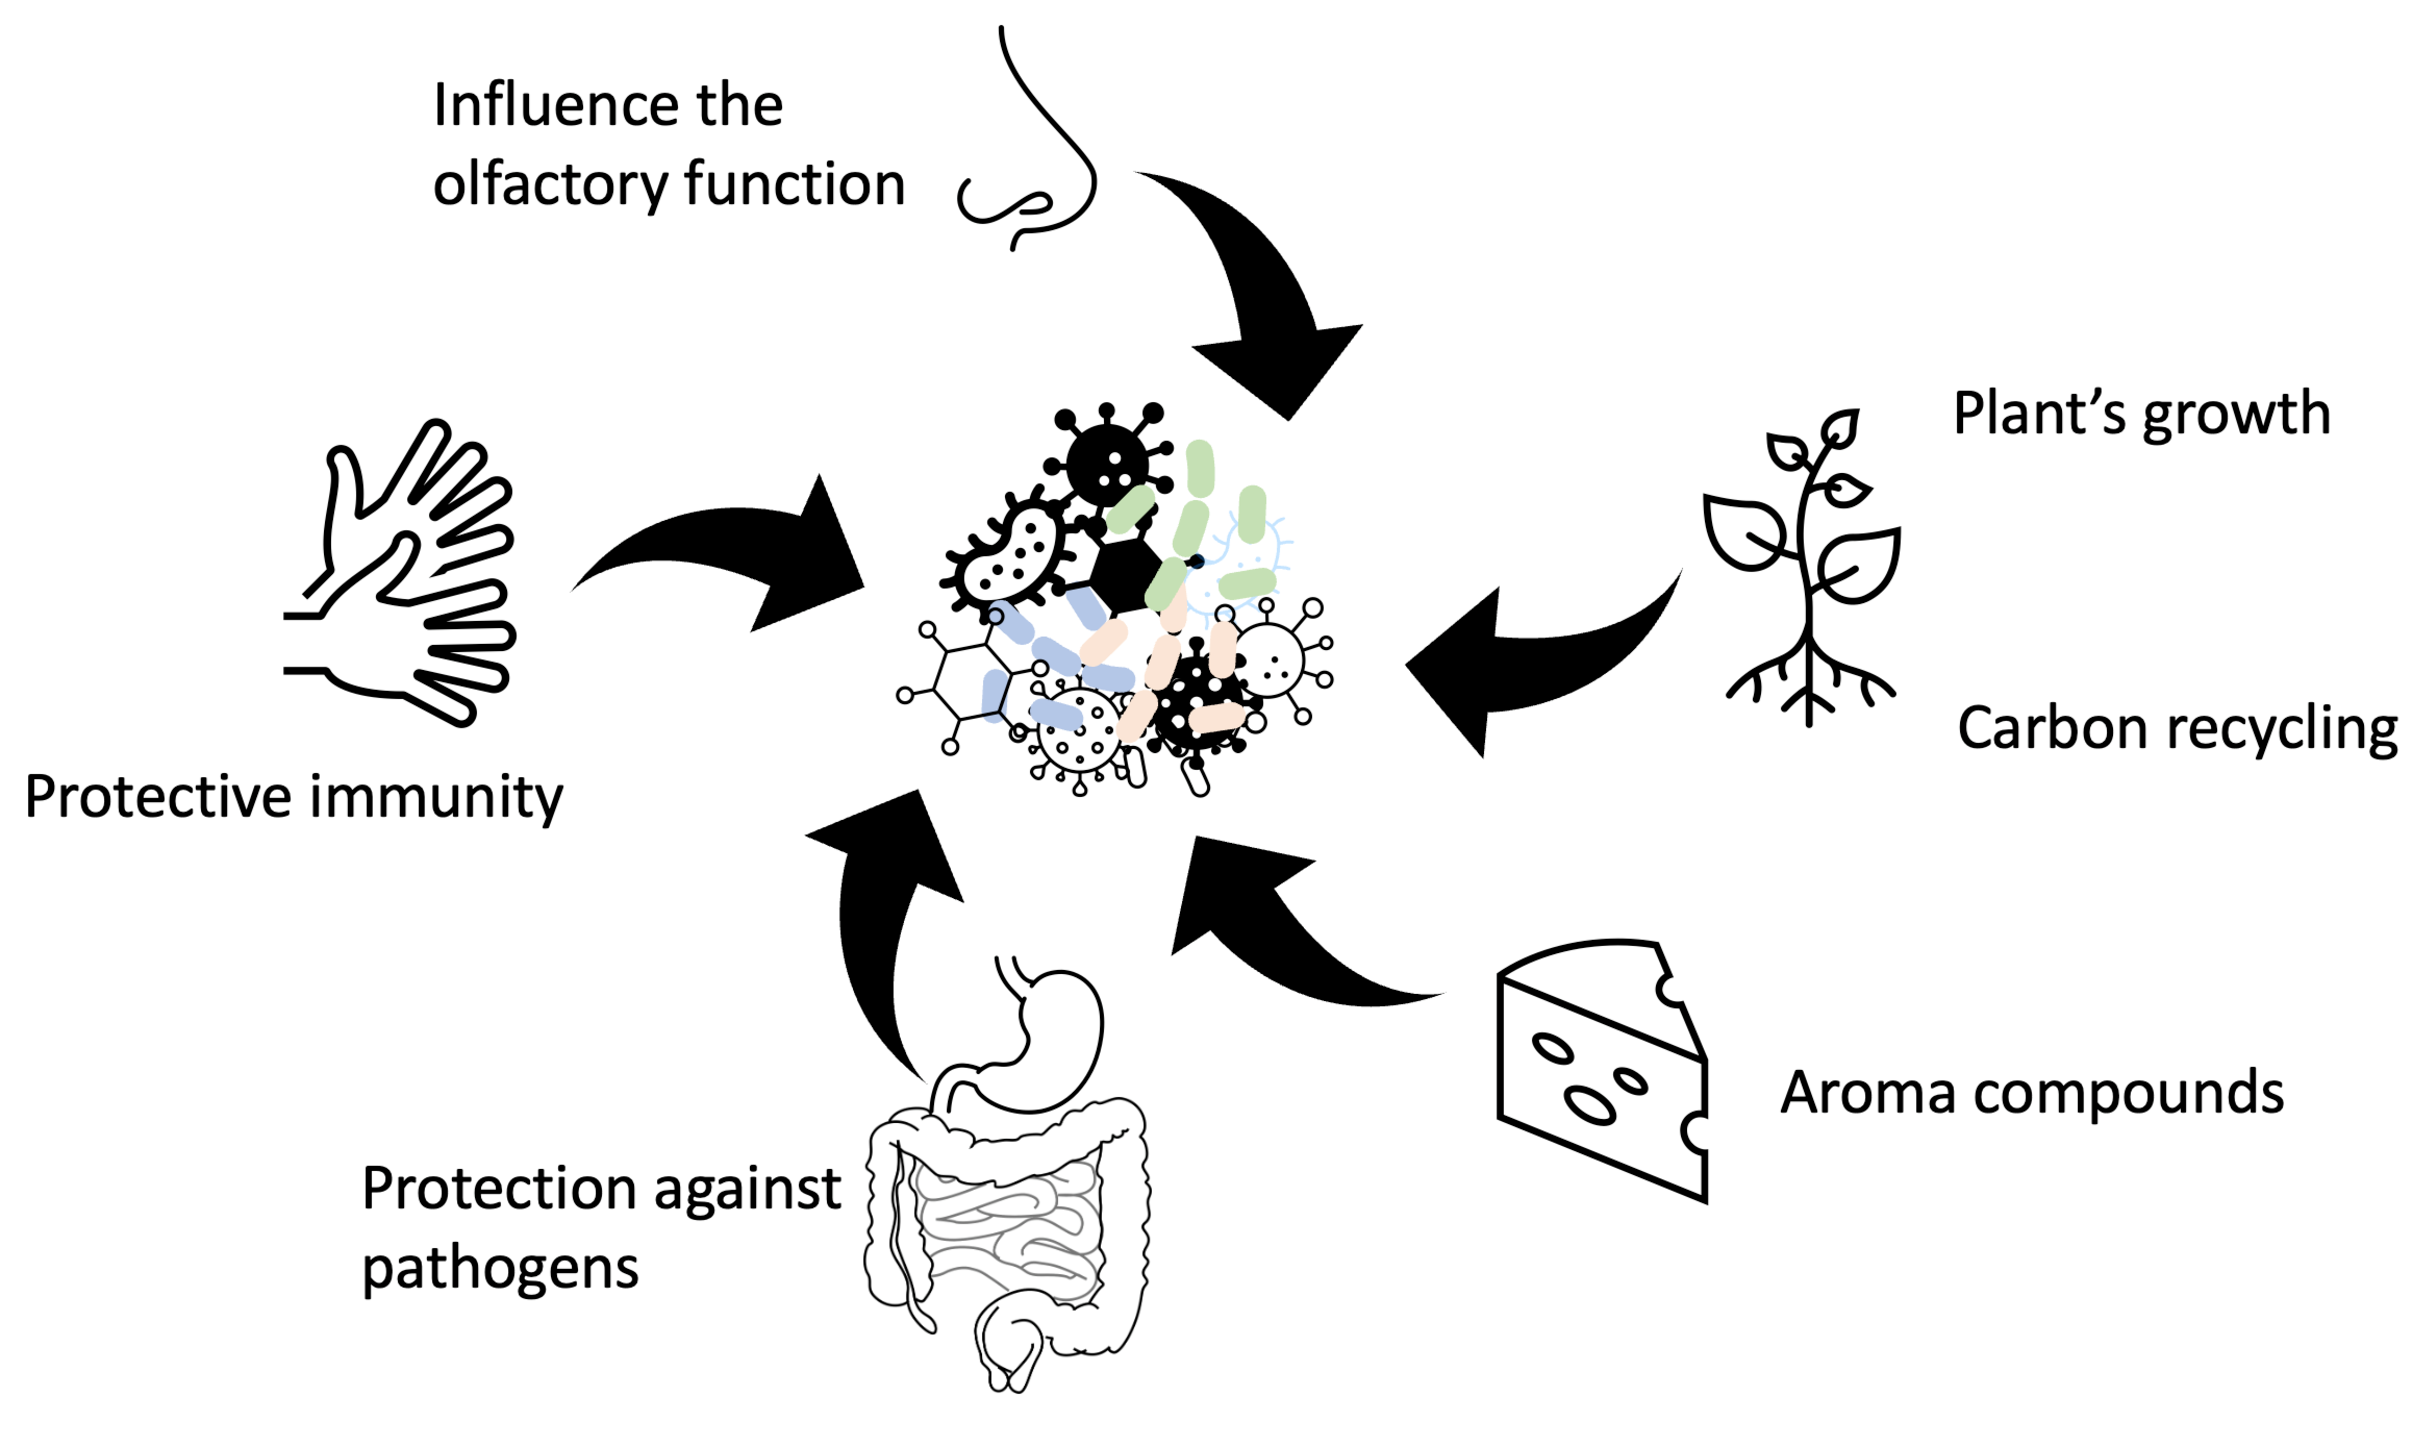
\includegraphics[width=0.9\textwidth]{figures/bacterial-env.pdf}
\end{figure}
\begin{block}{}
\begin{itemize}
\item High diversity of microorganisms
\item Microorganisms roles specific to the environment \tiny\citep{10.1093/chemse/bjh067,BELKAID2014121,Zhang2015,Hoorman2011,McSweeney2000}
\end{itemize}
\end{block}
\end{frame}

\begin{frame}
\frametitle{Bacterial interaction are responsible of the observed roles}

\begin{figure}
	\centering
	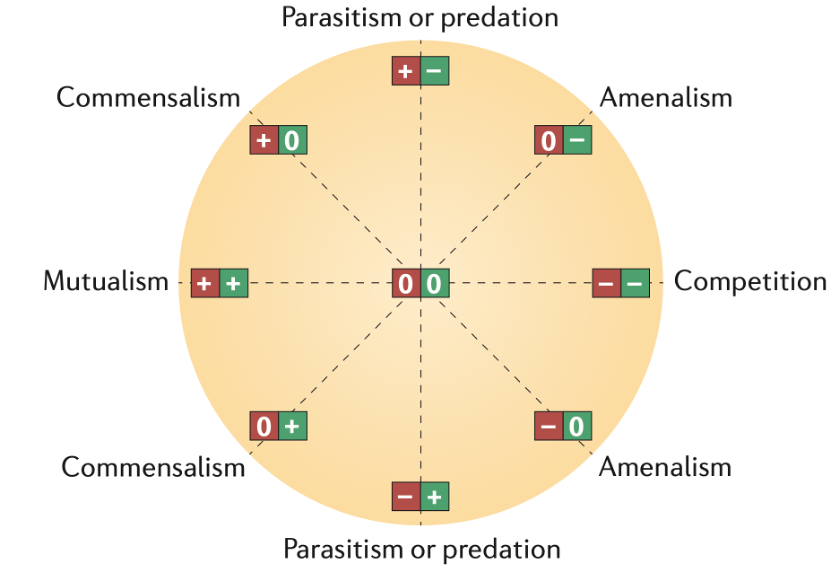
\includegraphics[width=0.8\textwidth]{figures/interaction.png}
    \caption{List of different types of bacterial interactions \tiny \citep{Faust2012} }
\end{figure}
\vspace{-0.5cm}
\begin{block}{}
\begin{itemize}
\item Bacterial interactions are distinguishable within two species
\item And within ecosystems composed of thousand of species ? $\rightarrow$ need of informatic 
\end{itemize}
\end{block}

\end{frame}


\begin{frame}
\frametitle{How can we combine biological knowledge and infomatic program ?}
\framesubtitle{Systems biology}
\begin{exampleblock}{System biology}
Associate an organism to a system and study the all system \tiny \citep{Kitano2002}
\end{exampleblock}
\begin{minipage}{0.8\textwidth}
\begin{figure}
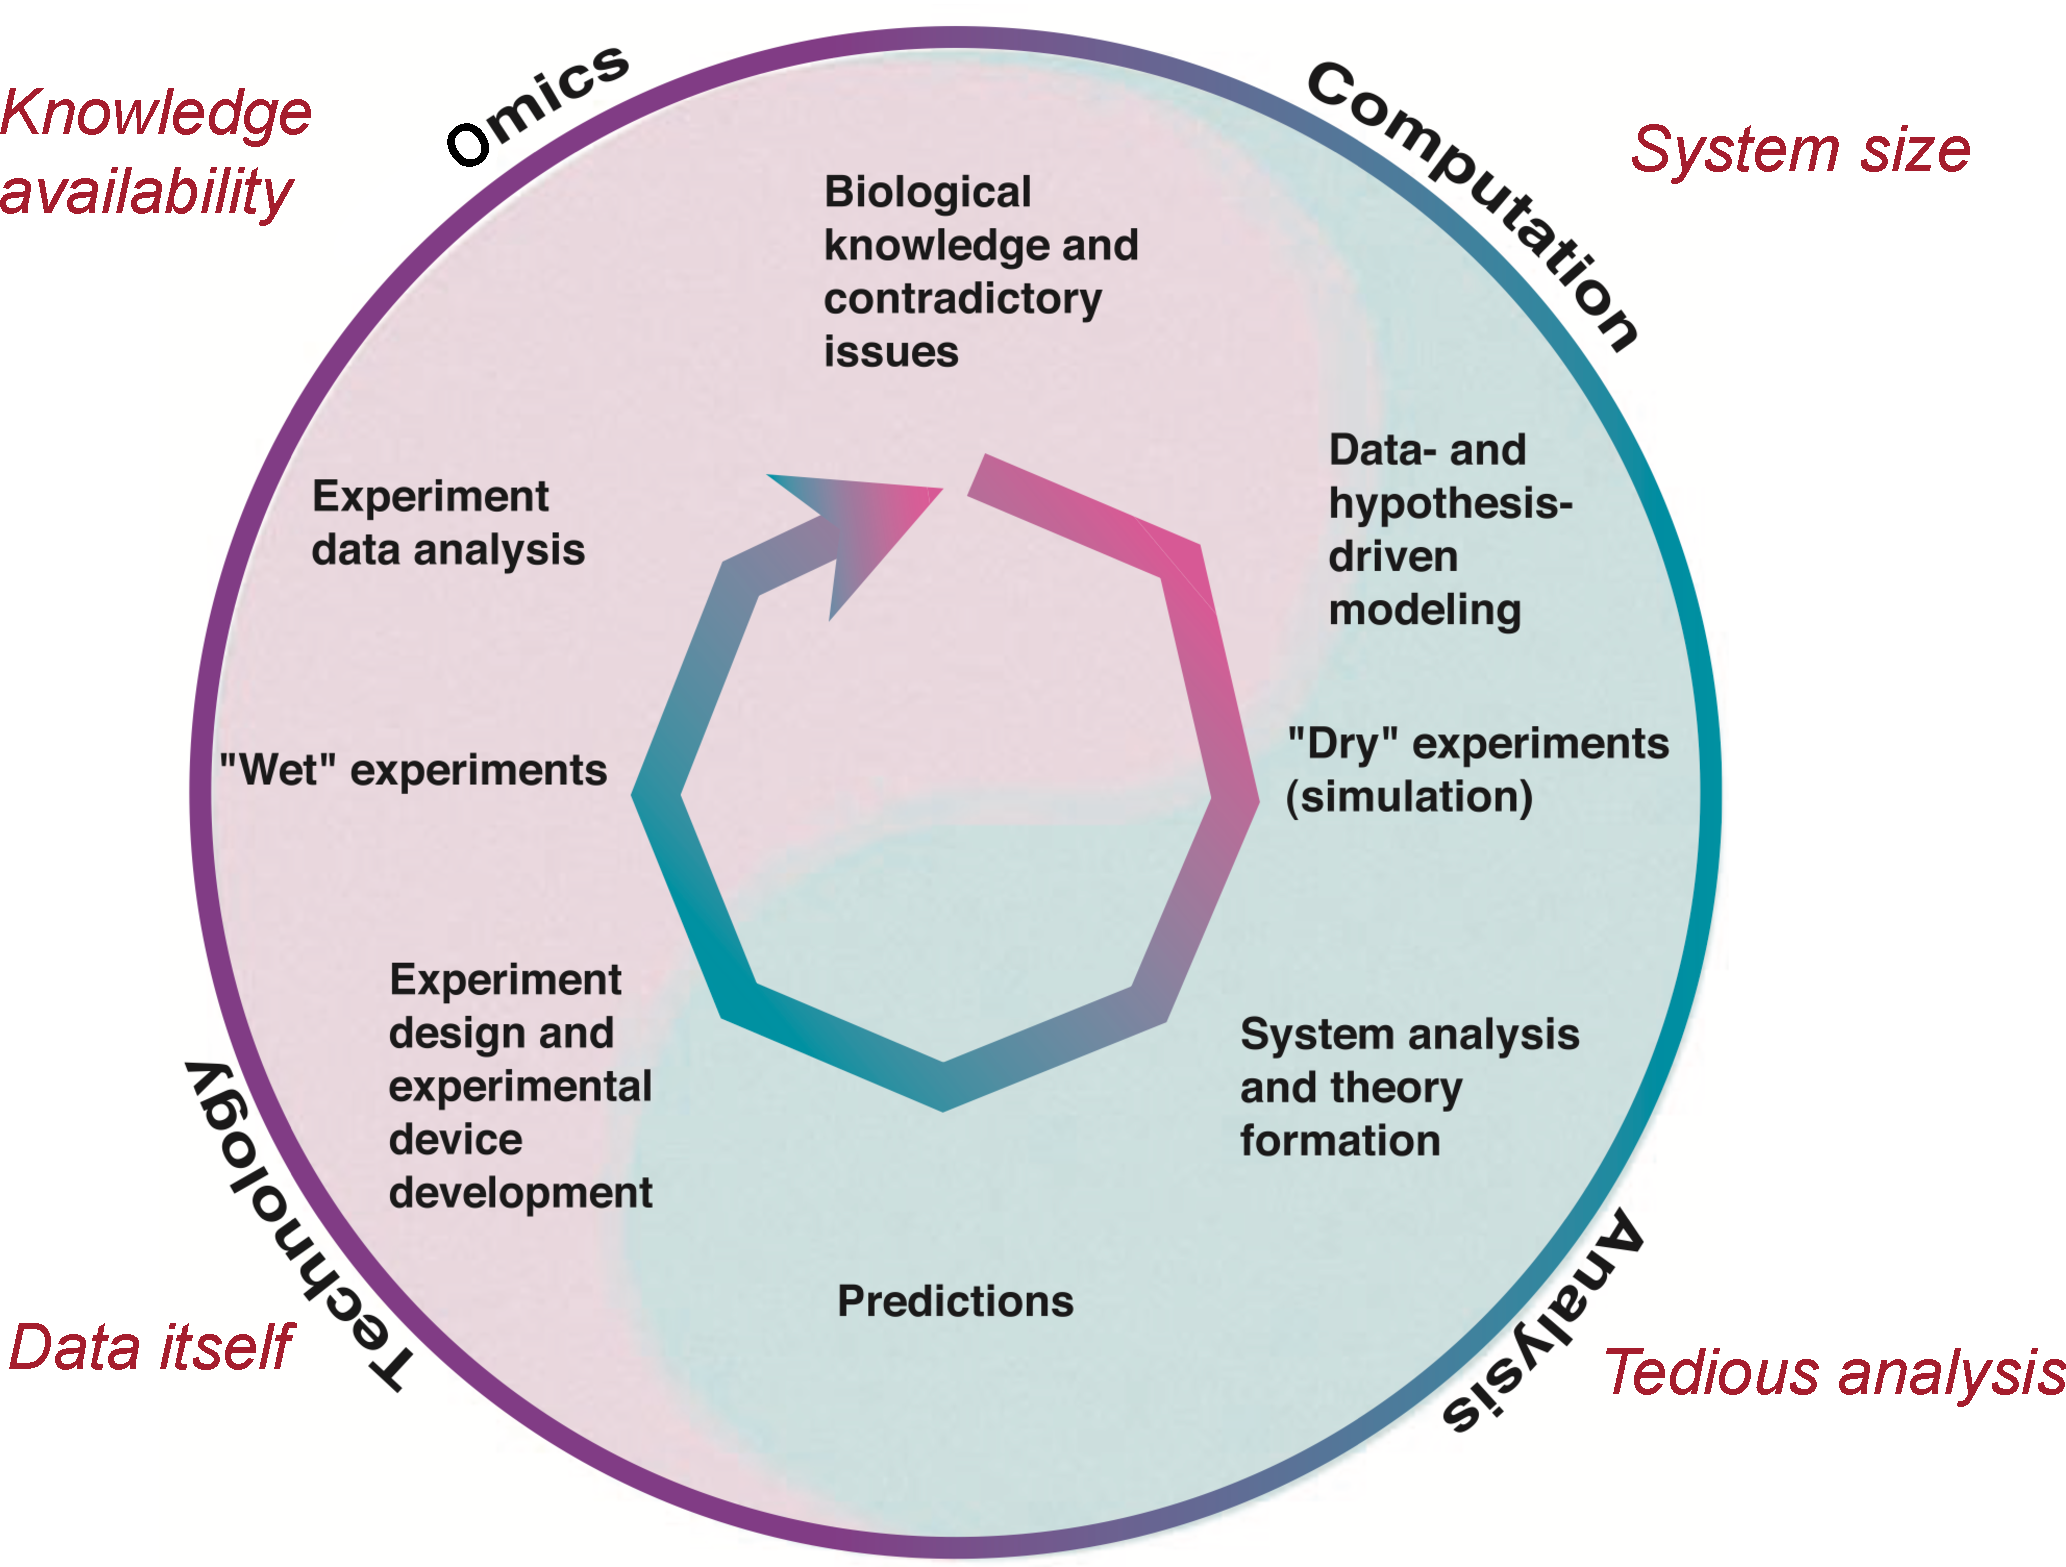
\includegraphics[width=0.9\textwidth]{figures/systeme-biology.pdf}
\caption{System biology modified from \cite{Kitano2002}}
\end{figure}
\end{minipage}%
\hspace{-1.1cm}%
\begin{minipage}{0.3\textwidth}
\begin{block}{}
\begin{itemize}
\item Which type of computation model is involved ?
\end{itemize}
\end{block}
\end{minipage}
\end{frame}



\begin{frame}
\frametitle{Metabolism as a starter pack for analysing bacterial interactions}
\only<1>{
\framesubtitle{Metabolism}
\vspace{-1.9cm}
\begin{figure}
	\centering
	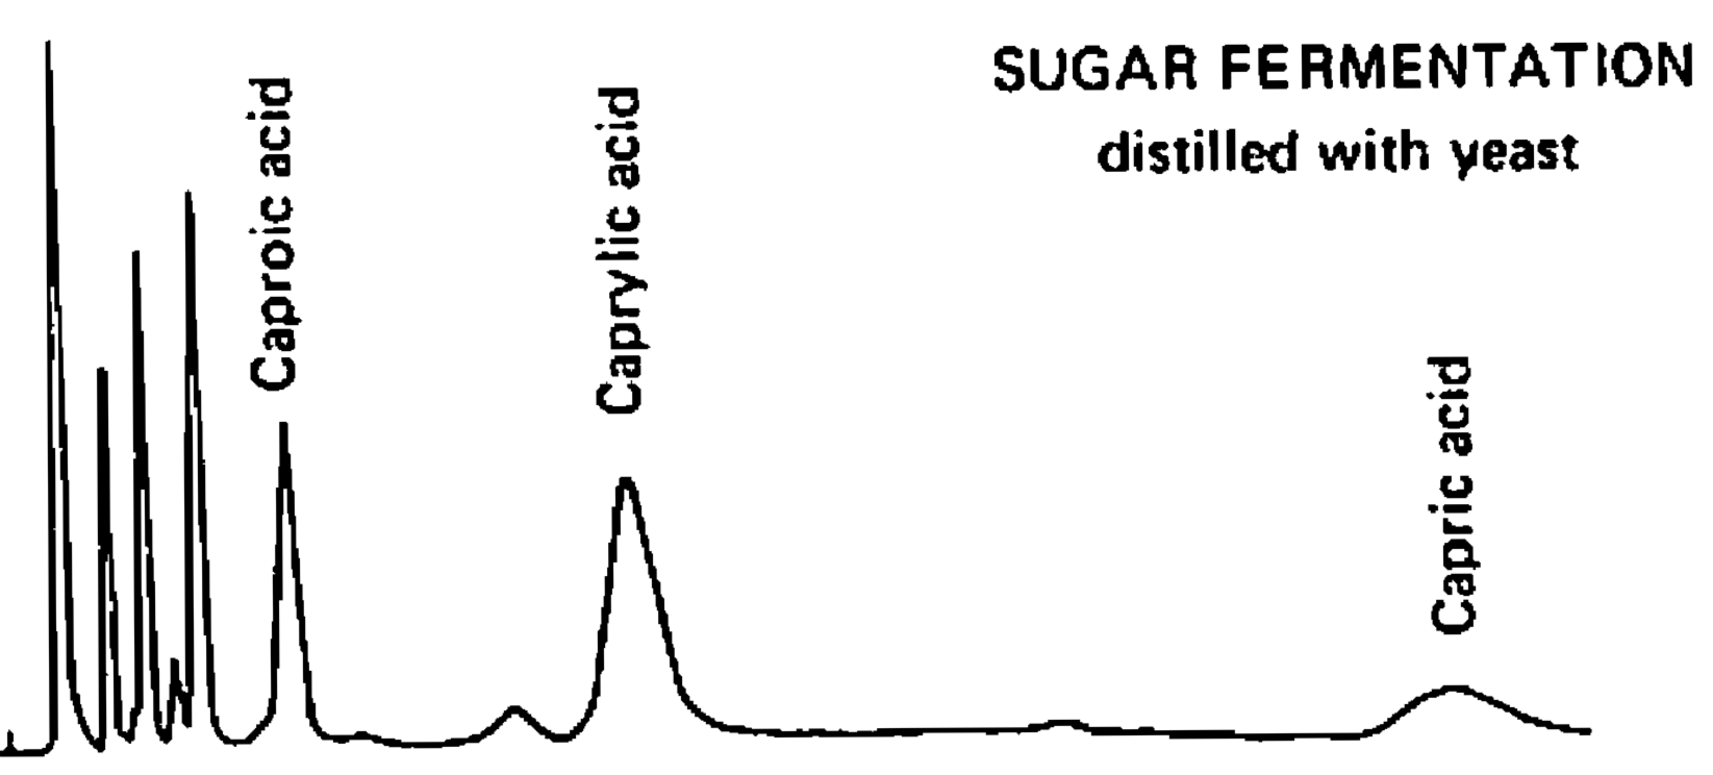
\includegraphics[width=0.7\textwidth]{figures/aroma-cpd-rum}
    \caption{Gas chromatograms of the major aroma compounds isolated from rum  \tiny (from \cite{Suomalainen1978})}
\end{figure}

}

\only<2>{
\framesubtitle{Metabolism}
\vspace{-1.1cm}
\begin{figure}
	\centering
	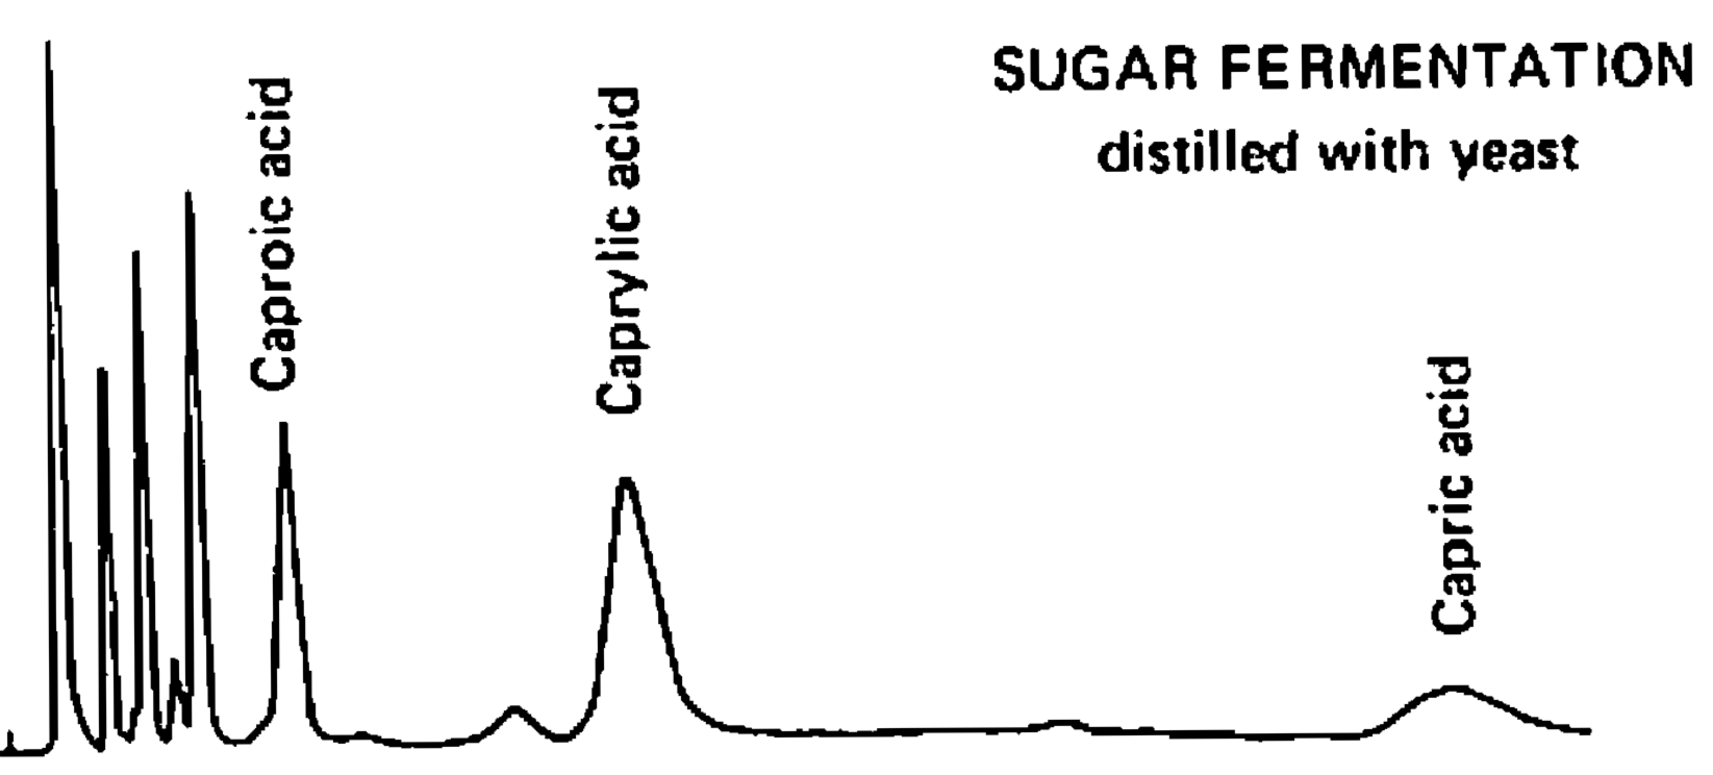
\includegraphics[width=0.7\textwidth]{figures/aroma-cpd-rum}
    \caption{Gas chromatograms of the major aroma compounds isolated from rum  \tiny (from \cite{Suomalainen1978})}
\end{figure}
\vspace{-0.7cm}
\begin{exampleblock}{What is metabolism ?}
Set of all biochemical reactions occurring in the cell of an organism that permit the production of energy and metabolic goods. \tiny \citep{Nava2023}
\end{exampleblock}

}

\only<3>{
\frametitle{What underlying mechanisms are responsible of the observed activity ?}
\framesubtitle{Metabolism and Bacterial interactions}
\vspace{-0.8cm}
\begin{figure}
	\centering
	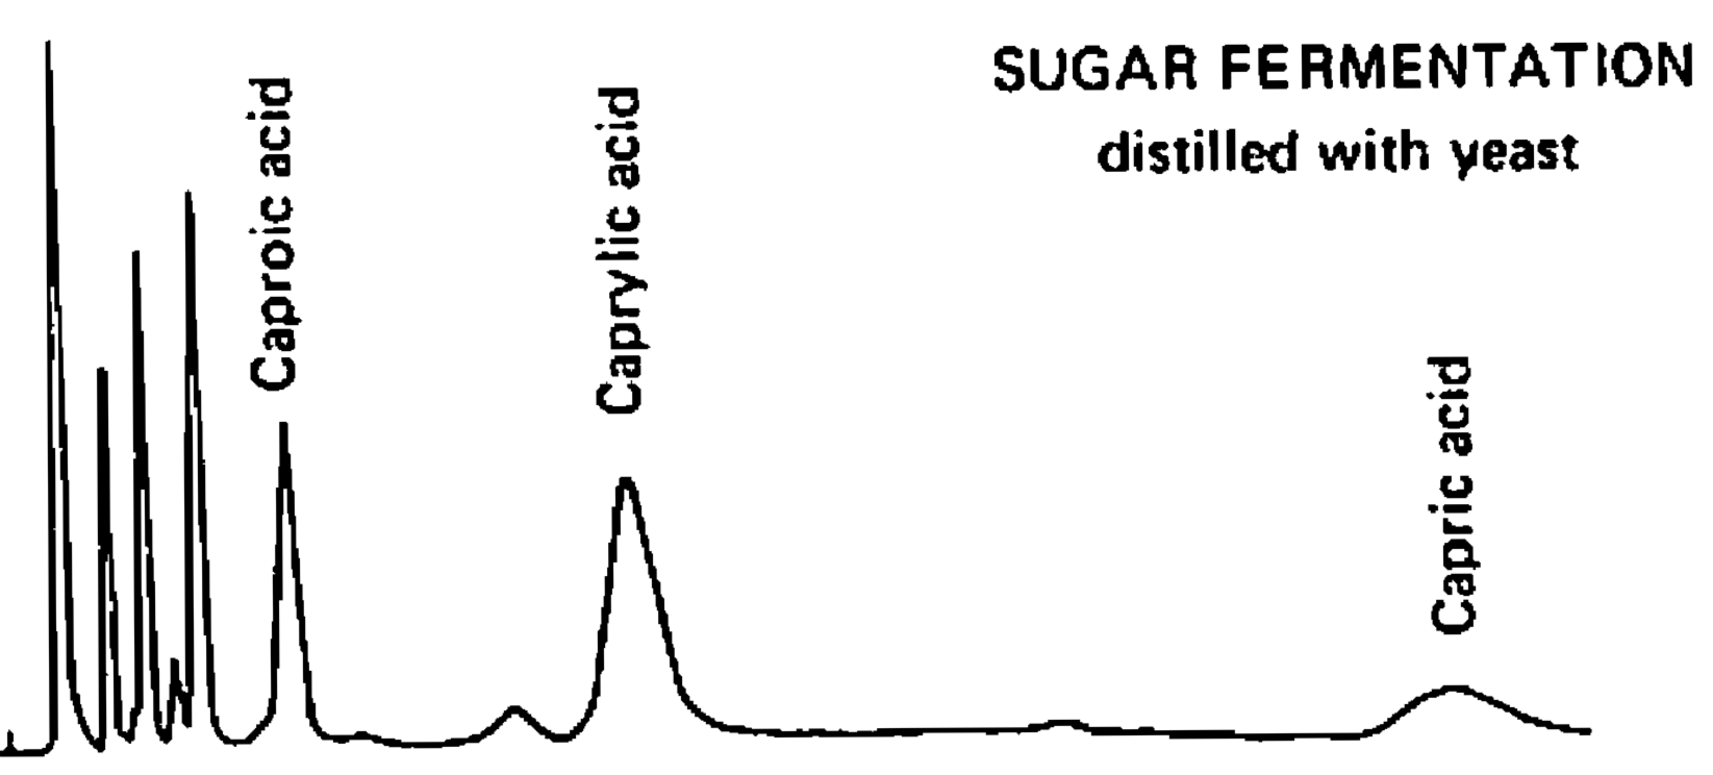
\includegraphics[width=0.7\textwidth]{figures/aroma-cpd-rum}
    \caption{Gas chromatograms of the major aroma compounds isolated from rum  \tiny (from \cite{Suomalainen1978})}
\end{figure}
\vspace{-0.5cm}
\begin{exampleblock}{What is metabolism ?}
Set of all biochemical reactions occurring in the cell of an organism that permit the production of energy and metabolic goods. \tiny \citep{Nava2023}
\end{exampleblock}
a fatty acyl-CoA + ethanol $\rightarrow$ ethyl palmitate + coA

}

\only<4>{
\frametitle{What underlying mechanisms are responsible of the observed activity ?}
\framesubtitle{Metabolism and Bacterial interactions}

\begin{figure}
	\centering
	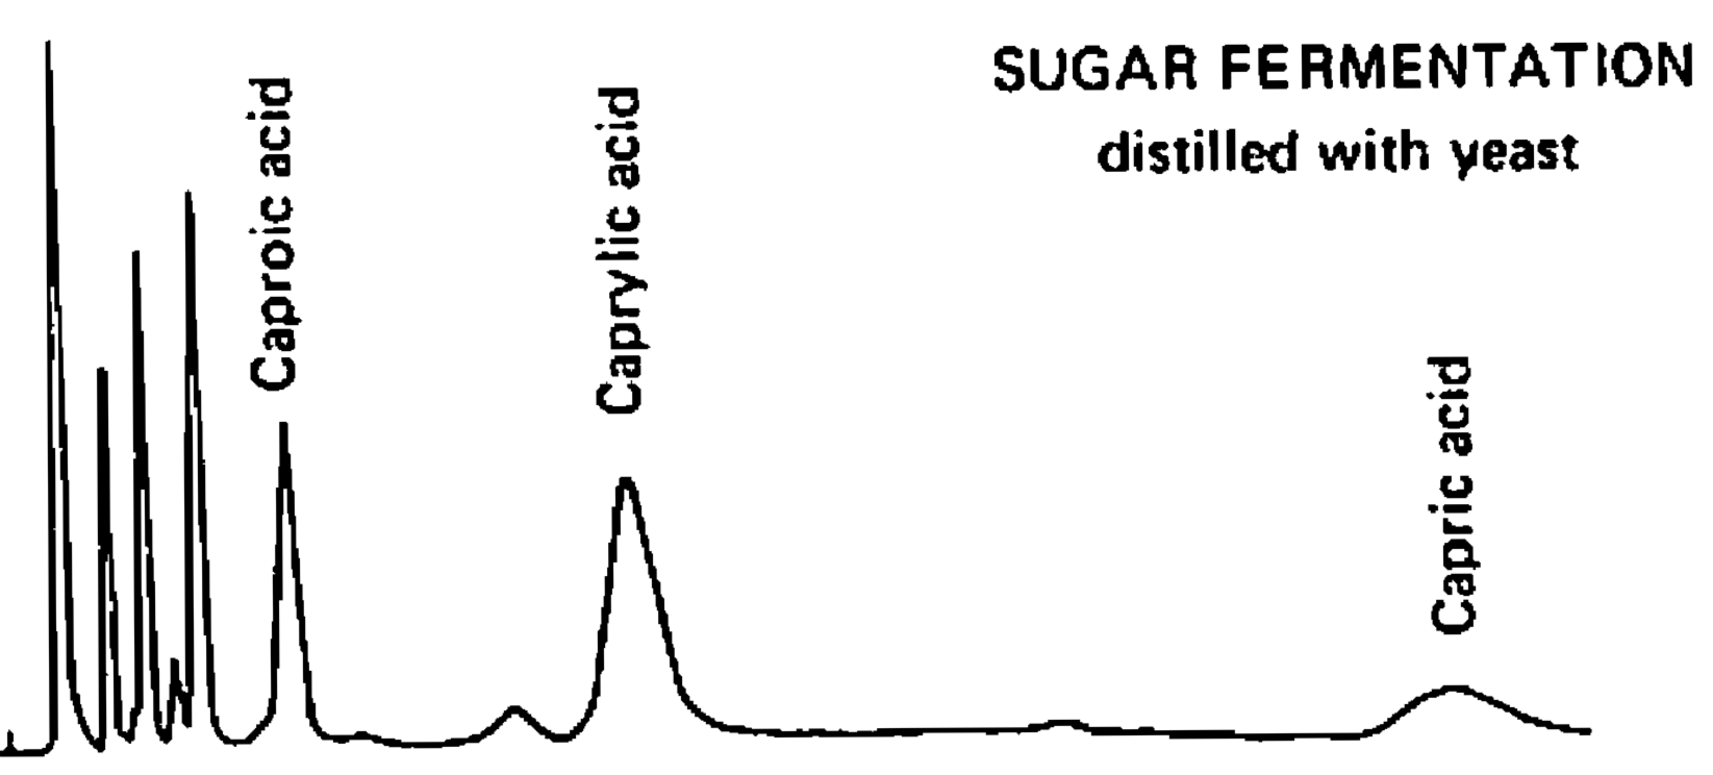
\includegraphics[width=0.7\textwidth]{figures/aroma-cpd-rum}
    \caption{Gas chromatograms of the major aroma compounds isolated from rum  \tiny (from \cite{Suomalainen1978})}
\end{figure}
\vspace{-0.5cm}
\begin{exampleblock}{What is metabolism ?}
Set of all biochemical reactions occurring in the cell of an organism that permit the production of energy and metabolic goods. \tiny \citep{Nava2023}
\end{exampleblock}
a fatty acyl-CoA + ethanol $\rightarrow$ ethyl palmitate + coA
\begin{block}{}
\begin{itemize}
\item Metabolism of an organism explain observable phenotype
\item Is impacted by bacterial interactions 
\end{itemize}
\end{block}

}
%
%\only<4>{
%\frametitle{What underlying mechanisms are responsible of the observed activity ?}
%\framesubtitle{Metabolism and Bacterial interactions}
%\begin{minipage}{0.4\textwidth}
%\begin{figure}
%	\centering
%	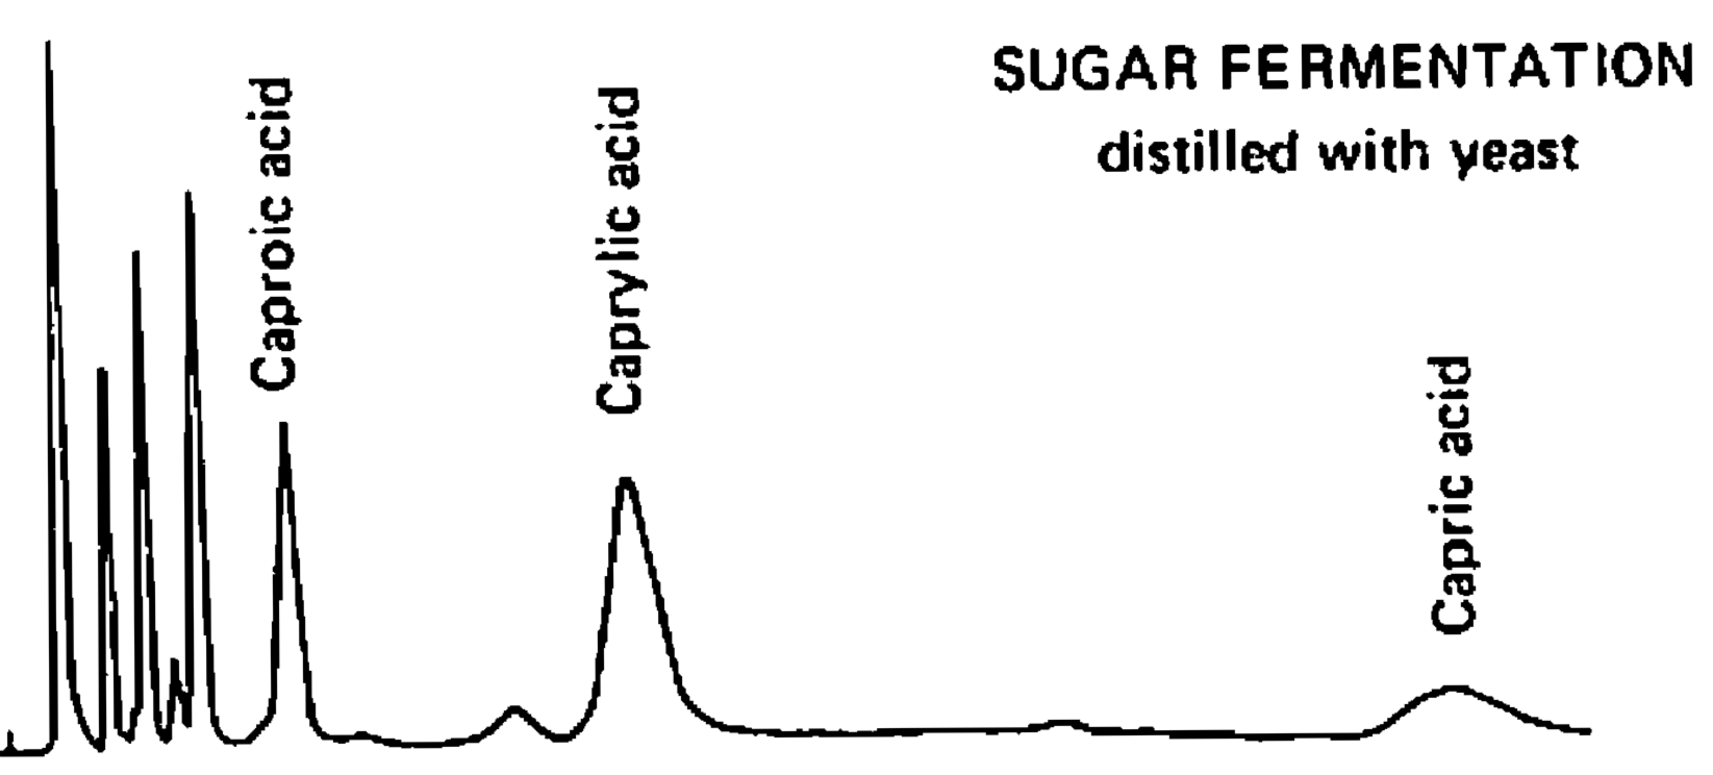
\includegraphics[width=0.9\textwidth]{figures/aroma-cpd-rum}
%    \caption{Gas chromatograms of the major aroma compounds isolated from rum  \tiny (from \cite{Suomalainen1978})}
%\end{figure}
%\vspace{-0.7cm}
%\begin{exampleblock}{What is metabolism ?}
%Set of all biochemical reactions occurring in the cell of an organism that permit the production of energy and metabolic goods. \tiny \citep{Nava2023}
%\end{exampleblock}
%a fatty acyl-CoA + ethanol $\rightarrow$ ethyl palmitate + coA
%\begin{itemize}
%\item Metabolism of an organism explain observable phenotype
%\end{itemize}
%\end{minipage}%
%\hspace{0.1\textwidth}%
%\begin{minipage}{0.5\textwidth}
%\begin{figure}
%	\centering
%	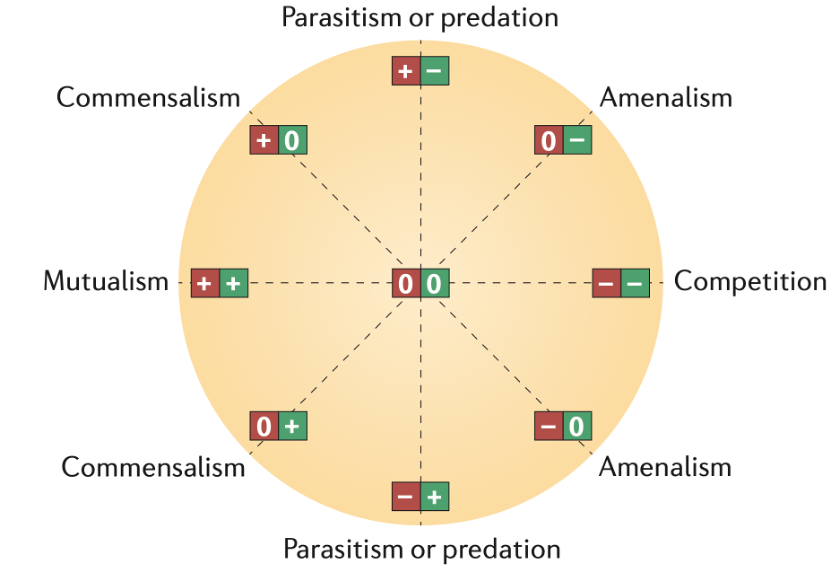
\includegraphics[width=\textwidth]{figures/interaction.png}
%    \caption{List of different types of bacterial interactions \tiny \citep{Faust2012} }
%\end{figure}
%\begin{itemize}
%\item Bacterial interaction can affect positively / negatively other organisms
%\end{itemize}
%\end{minipage}
%}
%
%\only<5>{
%\frametitle{What underlying mechanisms are responsible of the observed activity ?}
%\framesubtitle{Metabolism and Bacterial interactions}
%\begin{minipage}{0.4\textwidth}
%\begin{figure}
%	\centering
%	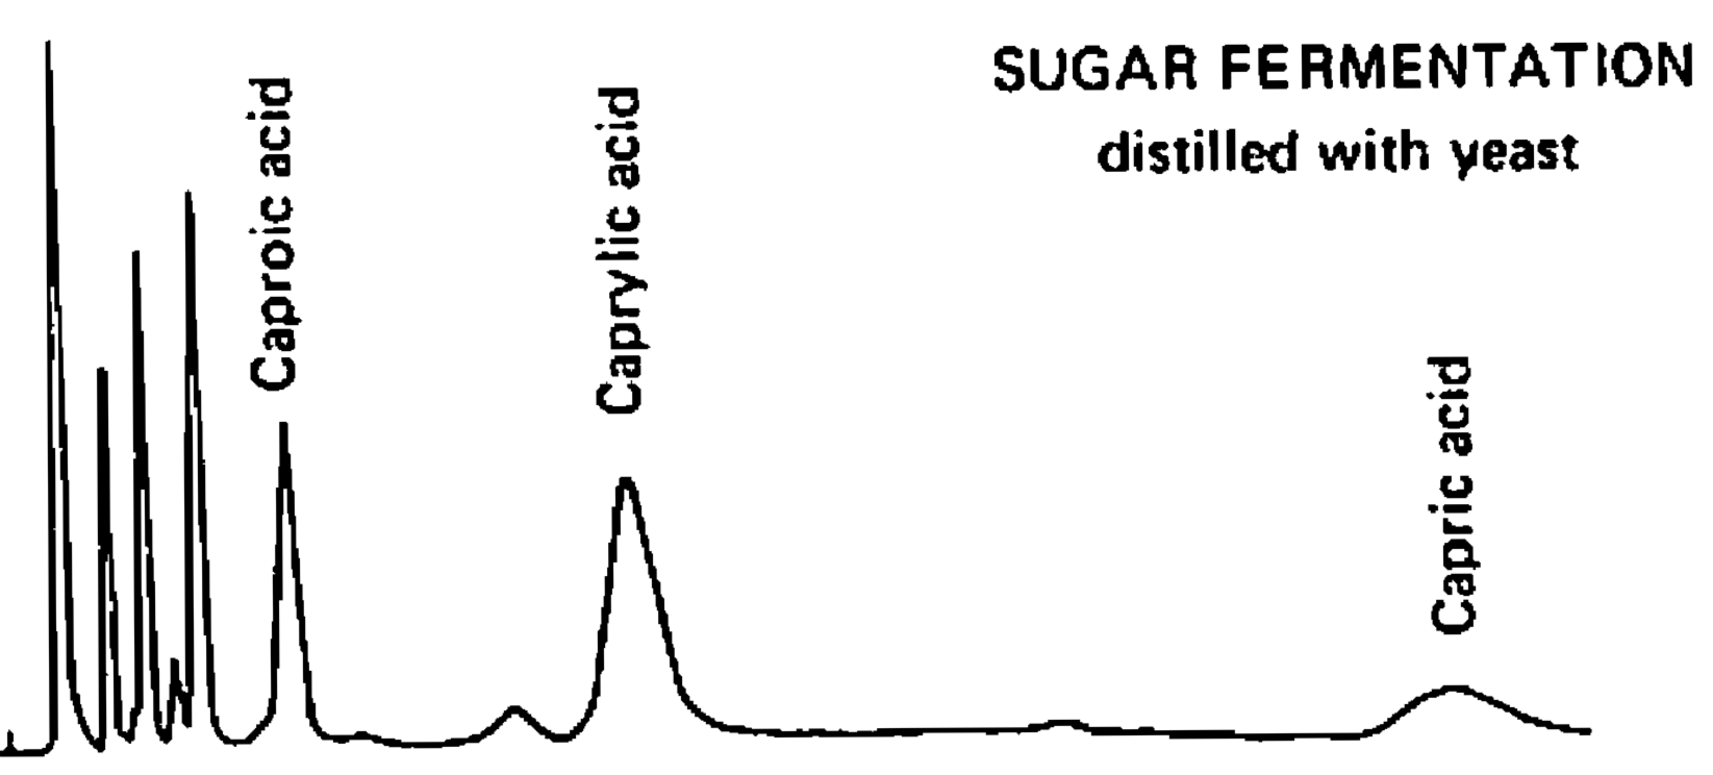
\includegraphics[width=0.9\textwidth]{figures/aroma-cpd-rum}
%    \caption{Gas chromatograms of the major aroma compounds isolated from rum  \tiny (from \cite{Suomalainen1978})}
%\end{figure}
%\vspace{-0.7cm}
%\begin{exampleblock}{What is metabolism ?}
%Set of all biochemical reactions occurring in the cell of an organism that permit the production of energy and metabolic goods. \tiny \citep{Nava2023}
%\end{exampleblock}
%a fatty acyl-CoA + ethanol $\rightarrow$ ethyl palmitate + coA
%\begin{itemize}
%\item Metabolism of an organism explain observable phenotype
%\end{itemize}
%\end{minipage}%
%\hspace{0.1\textwidth}%
%\begin{minipage}{0.5\textwidth}
%\begin{figure}
%	\centering
%	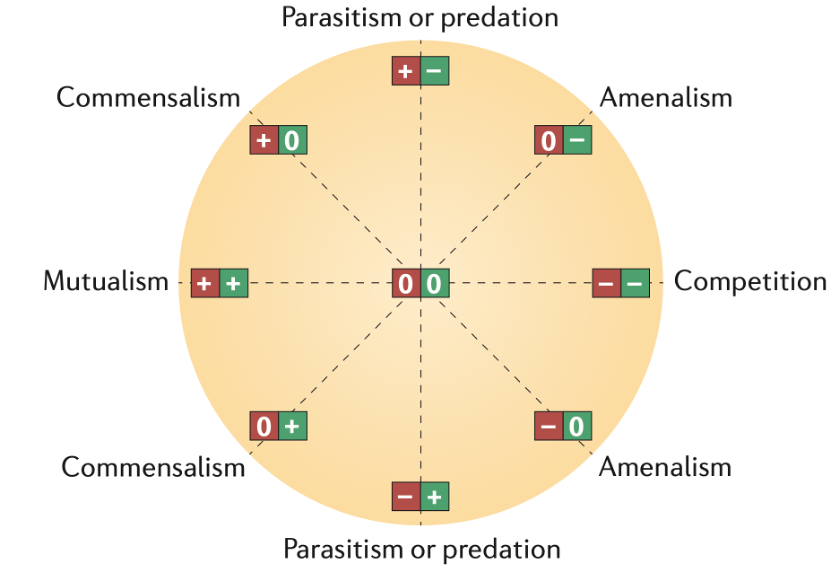
\includegraphics[width=\textwidth]{figures/interaction.png}
%    \caption{List of different types of bacterial interactions \tiny \citep{Faust2012} }
%\end{figure}
%\begin{itemize}
%\item Bacterial interaction can affect positively / negatively other organisms
%\end{itemize}
%\end{minipage}
%\begin{block}{}
%
%Bacterial interactions can modulate metabolic goods
%
%\end{block}}
\end{frame}

\section{Background}
\begin{frame}
\frametitle{How is the metabolism represented?}
\only<1>{
\vspace{-2.5cm}
$r_1 : $2 pyr $\rightarrow$ 1 acetoL + 1 $\text{CO}_2$ \\
$r_2 : $1 aceto-Lac  $\rightarrow$ 1 diac  + 1 $\text{CO}_2$ \\ 
$r_3 : $1 aceto-Lac  $\rightarrow$ 1 acetoin + 1 $\text{CO}_2$ \\
$r_4 : $1 diac $\rightarrow$ 1 acetoin \\
$r_5 : $1 acetoin  $\rightarrow$1 butanediol \\

}

\only<2>{
\begin{minipage}{0.5\textwidth}
$r_1 : $2 pyr $\rightarrow$ 1 acetoL + 1 $\text{CO}_2$ \\
$r_2 : $1 aceto-Lac  $\rightarrow$ 1 diac  + 1 $\text{CO}_2$ \\ 
$r_3 : $1 aceto-Lac  $\rightarrow$ 1 acetoin + 1 $\text{CO}_2$ \\
$r_4 : $1 diac $\rightarrow$ 1 acetoin \\
$r_5 : $1 acetoin  $\rightarrow$1 butanediol \\


\textbf{Stoichiometry matrix}


\[
  \kbordermatrix{
     & r_1  & r_2 & r_3 & r_4 & r_5 \\
    \text{pyr}                                           & -2 & 0 & 0 & 0 & 0 \\
    \text{aceto-Lac}                      & 1 & -1 & -1 & 0 & 0  \\
    \text{diac}                      & 0 & 1 & 0 & -1 & 0  \\
    \text{CO}_2         & 1 & 1 & 1 & 0 & 0    \\
    \text{acetoin}         & 0 & 0 & 1 & 1 & -1   \\
    \text{butanediol}         & 0 & 0 & 0 & 0 & 1  \\
        }
\]


\end{minipage}%
\begin{minipage}{0.5\textwidth}


\end{minipage}
}

\only<3>{
\begin{minipage}{0.5\textwidth}
$r_1 : $2 pyr $\rightarrow$ 1 acetoL + 1 $\text{CO}_2$ \\
$r_2 : $1 aceto-Lac  $\rightarrow$ 1 diac  + 1 $\text{CO}_2$ \\ 
$r_3 : $1 aceto-Lac $\rightarrow$ 1 acetoin + 1 $\text{CO}_2$ \\
$r_4 : $1 diac $\rightarrow$ 1 acetoin \\
$r_5 : $1 acetoin  $\rightarrow$1 butanediol \\

\textbf{Stoichiometry matrix}
\[
  \kbordermatrix{
     & r_1  & r_2 & r_3 & r_4 & r_5 \\
    \text{pyr}                                           & -2 & 0 & 0 & 0 & 0 \\
    \text{aceto-Lac}                      & 1 & -1 & -1 & 0 & 0  \\
    \text{diac}                      & 0 & 1 & 0 & -1 & 0  \\
    \text{CO}_2         & 1 & 1 & 1 & 0 & 0    \\
    \text{acetoin}         & 0 & 0 & 1 & 1 & -1   \\
    \text{butanediol}         & 0 & 0 & 0 & 0 & 1  \\
        }
\]
\end{minipage}%
\begin{minipage}{0.5\textwidth}
\centering
\textbf{bipartite graph}


\begin{tikzpicture}
\node (x) [circle, draw,mystyle] at (3,8)   {pyr};
  \node (a) [circle, draw,mystyle] at (4.5,6.8)   {aceto-Lac};
    \node (b) [circle, draw,mystyle] at (4.5,4.4)   {diac};
      \node (c) [circle, draw,mystyle] at (6,6.8)   {$ \text{CO}_2 $};
        \node (d) [circle, draw,mystyle] at (4.5,3)   {acetoin};
          \node (e) [circle, draw,mystyle] at (8,3)   {butanediol};
          
  \node (f) [rectangle, draw] at (4.5,8) {$r_1$};
  	\node (g) [rectangle, draw] at (4.5,5.6)  {$r_2$};
  	  \node (h) [rectangle, draw] at (6,4.4)   {$r_3$};
  		\node (i) [rectangle, draw] at (3,4.4)   {$r_4$};
  		  \node (j) [rectangle, draw] at (6,3)   {$r_5$};

  \graph { (x) -> (f) -> (a) };
   \graph { (x) -> (f) -> (c) };
   \graph { (a) -> (g) -> (c) };
    \graph { (a) -> (g) -> (b) };
	\graph { (b) -> (h) -> (c) };      
	 \graph { (b) -> (h) -> (d) };            
	 	 \graph { (b) -> (i) -> (d) };       
	 	 	 	 \graph { (d) -> (j) -> (e) };                 
	 
\end{tikzpicture}

\end{minipage}

\begin{block}{}
\textbf{Stoichiometry matrix} is commonly used for quantitative analysis instead of \textbf{graph}, more focused on topology analysis
\end{block}


}


 \end{frame}

\begin{frame}
\frametitle{How is the metabolism reconstructed?}
\framesubtitle{Genome-scale metabolic network (GSMN) reconstruction}
\vspace{-0.3cm}
\begin{exampleblock}{Genome-scale metabolic network (GSMNs)}
Contain metabolic reactions predicted from the entire genomic content through gene-protein-reaction (GPR) relationships \tiny \citep{Thiele.2010}
\end{exampleblock}
\begin{minipage}{0.3\textwidth}
\begin{align*}
    r1 : (g1 \land g2) \lor (g1 \land g3)
\end{align*}
\begin{align*}
    r2 : g1 \land (g2 \lor g3)
\end{align*}

Example of trivial boolean GPR relationship

\end{minipage}%
\begin{minipage}{0.7\textwidth}
\begin{figure}
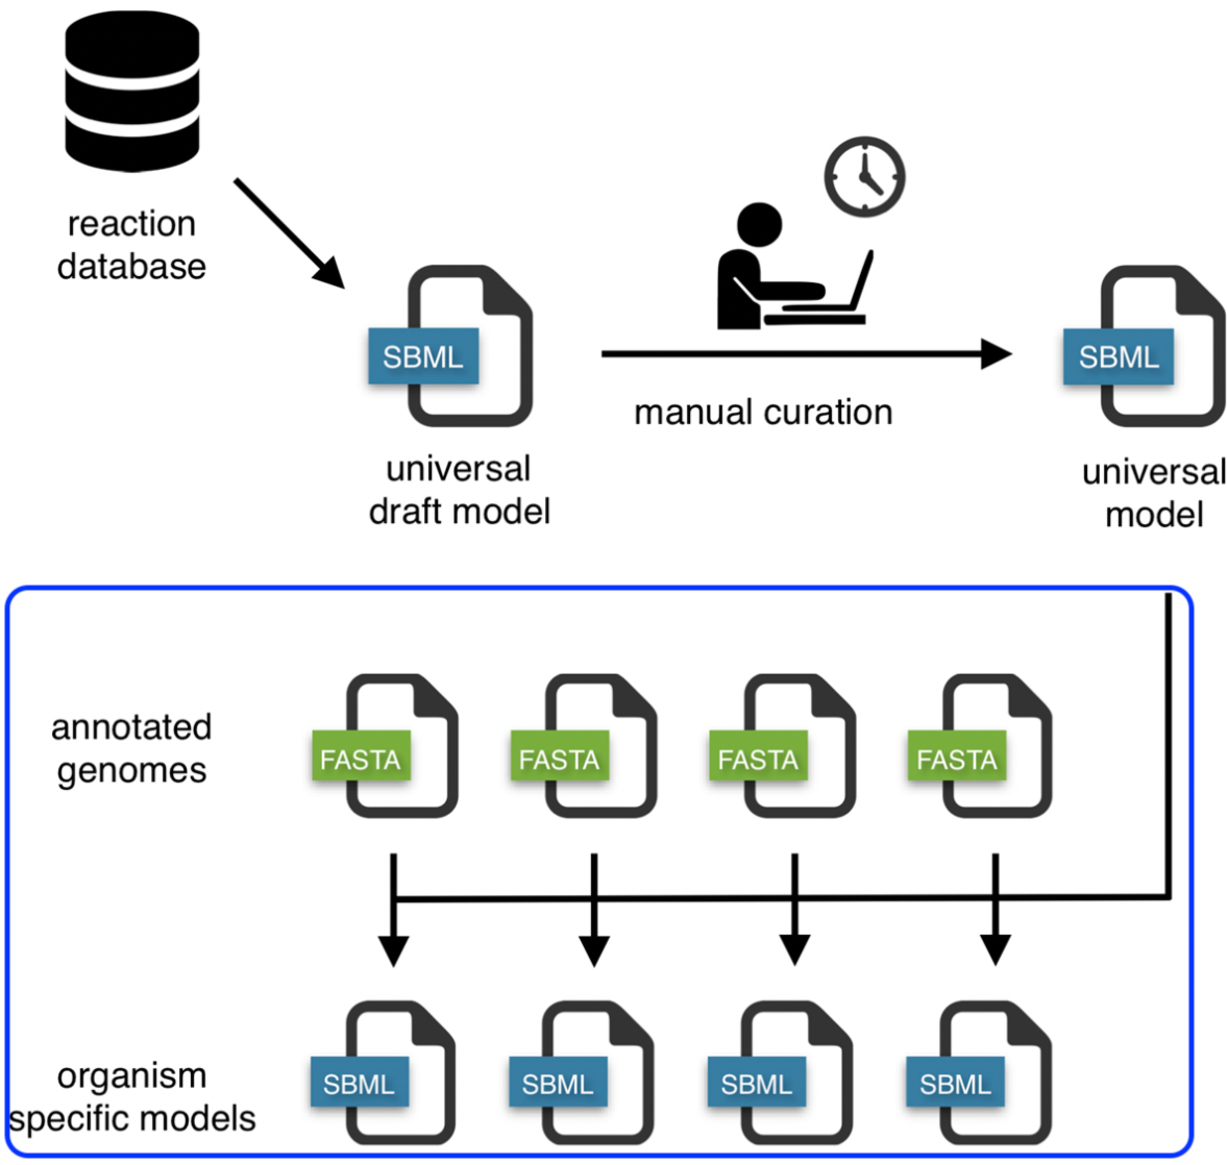
\includegraphics[width=0.7\textwidth]{figures/top-down}
\caption{Top down genome-scale metabolic network reconstruction approach \tiny (modified from \cite{Machado2018})}
\end{figure}
\end{minipage}
\vspace{-0.4cm}
\begin{block}{}
\begin{itemize}
\item For bacteria: average of 2000 reactions, 1200 genes, 1000 metabolites
\item Informatic can help to resolve combinatorial problem
\end{itemize}
\end{block}
\end{frame}




\begin{frame}
%[fragile]
%[containsverbatim]
\frametitle{Reasoning-based metabolic analysis}

\begin{onlyenv}<1>
\framesubtitle{Definition}
\vspace{-3cm}
\begin{exampleblock}{Reasoning-based}
Allow us to infer qualitative models from logical rules based on biological knowledge
\end{exampleblock}
\end{onlyenv}

\begin{onlyenv}<2>
\begin{exampleblock}{Reasoning-based}
Allow us to infer qualitative models from logical rules based on biological knowledge
\end{exampleblock}
\textbf{topological-based approaches}\\
\begin{minipage}{0.5\textwidth}
\hspace{-0.15\textwidth}
\begin{tikzpicture}
   \node (x) [circle, draw] at (0,0)   {X};
   \node (a) [circle, draw] at (2,0)   {A};
   \node (b) [circle, draw] at (4,0)   {C};
   \node (c) [circle, draw] at (3,1)   {D};
   \node (d) [circle, draw] at (5,-1)   {E};
   \node (e) [circle, draw] at (3.5,-2)   {F};
          
    \node (f) [rectangle, draw] at (1,0) {$r_1$};
  	\node (g) [rectangle, draw] at (3,0)  {$r_2$};
  	\node (h) [rectangle, draw] at (5,0)   {$r_3$};
  	\node (i) [rectangle, draw] at (4,-1)   {$r_4$};
  	\node (j) [rectangle, draw] at (5,-2)   {$r_5$};

    \graph { (x) -> (f) -> (a) };
    \graph { (x) -> (f) -> (c) };
    \graph { (a) -> (g) -> (c) };
    \graph { (a) -> (g) -> (b) };
	\graph { (b) -> (h) <-> (c) };
	\graph { (b) -> (h) -> (d) };            
	\graph { (b) <- (i) <- (d) };       
	\graph { (d) <- (j) <- (e) };               
\end{tikzpicture}

\begin{block}{}
How to compute metabolic capability ?
\end{block}
\end{minipage}%
\end{onlyenv}

\begin{onlyenv}<3>
\begin{exampleblock}{Reasoning-based}
Allow us to infer qualitative models from logical rules based on biological knowledge
\end{exampleblock}
\textbf{topological-based approaches}
\begin{minipage}{0.5\textwidth}
\hspace{-0.15\textwidth}
\begin{tikzpicture}
   \node (x) [circle, draw] at (0,0)   {X};
   \node (a) [circle, draw] at (2,0)   {A};
   \node (b) [circle, draw] at (4,0)   {C};
   \node (c) [circle, draw] at (3,1)   {D};
   \node (d) [circle, draw] at (5,-1)   {E};
   \node (e) [circle, draw] at (3.5,-2)   {F};
          
    \node (f) [rectangle, draw] at (1,0) {$r_1$};
  	\node (g) [rectangle, draw] at (3,0)  {$r_2$};
  	\node (h) [rectangle, draw] at (5,0)   {$r_3$};
  	\node (i) [rectangle, draw] at (4,-1)   {$r_4$};
  	\node (j) [rectangle, draw] at (5,-2)   {$r_5$};

    \graph { (x) -> (f) -> (a) };
    \graph { (x) -> (f) -> (c) };
    \graph { (a) -> (g) -> (c) };
    \graph { (a) -> (g) -> (b) };
	\graph { (b) -> (h) <-> (c) };
	\graph { (b) -> (h) -> (d) };            
	\graph { (b) <- (i) <- (d) };       
	\graph { (d) <- (j) <- (e) };               
\end{tikzpicture}
\end{minipage}%
\begin{minipage}{0.55\textwidth}
\begin{itemize}
\item Producibility is initiated by the presence of nutrients,
\item The products of a reactions are producible if all reactants of this reaction are themselves producible
\end{itemize}
%
%\begin{lstlisting}[style=asp]
%scope(M) :- seed(M).
%scope(M) :- bacteria(B), product(M,R,B), reaction(R,B), scope(M2) : reactant(M2,R,B).
%\end{lstlisting}
\end{minipage}

\begin{block}{}
The scope, \textit{i.e.} the metabolic capacity,  a network is reached in 2 logical rules \tiny \citep{Ebenhoh2004}
\end{block}
\end{onlyenv}
\end{frame}

\begin{frame}
\frametitle{Reasoning-based metabolic analysis}
\begin{exampleblock}{Reasoning-based}
Allow us to infer qualitative models from logical rules based on biological knowledge
\end{exampleblock}
\textbf{topological-based approaches}
\only<1> {
\begin{center}
\begin{tikzpicture}
   \node (x) [circle, draw,fill=black!30!yellow] at (0,0)   {X};
   \node (a) [circle, draw] at (2,0)   {A};
   \node (b) [circle, draw] at (4,0)   {C};
   \node (c) [circle, draw] at (3,1)   {D};
   \node (d) [circle, draw] at (5,-1)   {E};
   \node (e) [circle, draw] at (3.5,-2)   {F};
          
    \node (f) [rectangle, draw] at (1,0) {$r_1$};
  	\node (g) [rectangle, draw] at (3,0)  {$r_2$};
  	\node (h) [rectangle, draw] at (5,0)   {$r_3$};
  	\node (i) [rectangle, draw] at (4,-1)   {$r_4$};
  	\node (j) [rectangle, draw] at (5,-2)   {$r_5$};
  
    \graph { (x) -> (f) -> (a) };
    \graph { (x) -> (f) -> (c) };
    \graph { (a) -> (g) -> (c) };
    \graph { (a) -> (g) -> (b) };
	\graph { (b) -> (h) <-> (c) };
	\graph { (b) -> (h) -> (d) };            
	\graph { (b) <- (i) <- (d) };            
	\graph { (d) <- (j) <- (e) };         
	    \graph { (e) -> (i) };
	
     \draw [draw=black] (0.5,1.5) rectangle (5.5,-2.5);     
     
     \node (extracellular) [] at (6.5,1.5) {\tiny \textit{extracellular}};
     \node (intracellular) [] at (4.5,01) {\tiny \textit{intracellular}};	

\end{tikzpicture}
\end{center}
X is a seed
}

\only<2> {
\begin{center}
\begin{tikzpicture}
   \node (x) [circle, draw,fill=black!30!yellow] at (0,0)   {X};
   \node (a) [circle, draw,fill=white!60!yellow] at (2,0)   {A};
   \node (b) [circle, draw] at (4,0)   {C};
   \node (c) [circle, draw,fill=white!60!yellow] at (3,1)   {D};
   \node (d) [circle, draw] at (5,-1)   {E};
   \node (e) [circle, draw] at (3.5,-2)   {F};
          
    \node (f) [rectangle, draw,fill=white!60!yellow] at (1,0) {$r_1$};
  	\node (g) [rectangle, draw] at (3,0)  {$r_2$};
  	\node (h) [rectangle, draw] at (5,0)   {$r_3$};
  	\node (i) [rectangle, draw] at (4,-1)   {$r_4$};
  	\node (j) [rectangle, draw] at (5,-2)   {$r_5$};

    \graph { (x) -> (f) -> (a) };
    \graph { (x) -> (f) -> (c) };
    \graph { (a) -> (g) -> (c) };
    \graph { (a) -> (g) -> (b) };
	\graph { (b) -> (h) <-> (c) };
	\graph { (b) -> (h) -> (d) };            
	\graph { (b) <- (i) <- (d) };             
	\graph { (d) <- (j) <- (e) };    
	    \graph { (e) -> (i) };
	
	     \draw [draw=black] (0.5,1.5) rectangle (5.5,-2.5);     
	     
	          \node (extracellular) [] at (6.5,1.5) {\tiny \textit{extracellular}};
     \node (intracellular) [] at (4.5,01) {\tiny \textit{intracellular}};	
\end{tikzpicture}
\end{center}
X is available;  $r_1$ is activated and A,D are producible

}

\only<3> {
\begin{center}
\begin{tikzpicture}
   \node (x) [circle, draw,fill=black!30!yellow] at (0,0)   {X};
   \node (a) [circle, draw,fill=white!60!yellow] at (2,0)   {A};
   \node (b) [circle, draw,fill=white!60!yellow] at (4,0)   {C};
   \node (c) [circle, draw,fill=white!60!yellow] at (3,1)   {D};
   \node (d) [circle, draw] at (5,-1)   {E};
   \node (e) [circle, draw] at (3.5,-2)   {F};
          
    \node (f) [rectangle, draw,fill=white!60!yellow] at (1,0) {$r_1$};
  	\node (g) [rectangle, draw,fill=white!60!yellow] at (3,0)  {$r_2$};
  	\node (h) [rectangle, draw] at (5,0)   {$r_3$};
  	\node (i) [rectangle, draw] at (4,-1)   {$r_4$};
  	\node (j) [rectangle, draw] at (5,-2)   {$r_5$};

    \graph { (x) -> (f) -> (a) };
    \graph { (x) -> (f) -> (c) };
    \graph { (a) -> (g) -> (c) };
    \graph { (a) -> (g) -> (b) };
	\graph { (b) -> (h) <-> (c) };
	\graph { (b) -> (h) -> (d) };            
	\graph { (b) <- (i) <- (d) };         
	\graph { (d) <- (j) <- (e) };               
	    \graph { (e) -> (i) };
	
	     \draw [draw=black] (0.5,1.5) rectangle (5.5,-2.5);     
	     
	          \node (extracellular) [] at (6.5,1.5) {\tiny \textit{extracellular}};
     \node (intracellular) [] at (4.5,01) {\tiny \textit{intracellular}};	
\end{tikzpicture}
\end{center}
A,D are available;  $r_2$ is activated and C is producible
}

\only<4>{
\begin{center}
\begin{tikzpicture}
   \node (x) [circle, draw,fill=black!30!yellow] at (0,0)   {X};
   \node (a) [circle, draw,fill=white!60!yellow] at (2,0)   {A};
   \node (b) [circle, draw,fill=white!60!yellow] at (4,0)   {C};
   \node (c) [circle, draw,fill=white!60!yellow] at (3,1)   {D};
   \node (d) [circle, draw,fill=white!60!yellow] at (5,-1)   {E};
   \node (e) [circle, draw] at (3.5,-2)   {F};
          
    \node (f) [rectangle, draw,fill=white!60!yellow] at (1,0) {$r_1$};
  	\node (g) [rectangle, draw,fill=white!60!yellow] at (3,0)  {$r_2$};
  	\node (h) [rectangle, draw,fill=white!60!yellow] at (5,0)   {$r_3$};
  	\node (i) [rectangle, draw] at (4,-1)   {$r_4$};
  	\node (j) [rectangle, draw] at (5,-2)   {$r_5$};
  	


    \graph { (x) -> (f) -> (a) };
    \graph { (x) -> (f) -> (c) };
    \graph { (a) -> (g) -> (c) };
    \graph { (a) -> (g) -> (b) };
	\graph { (b) -> (h) <-> (c) };
	\graph { (b) -> (h) -> (d) };            
	\graph { (b) <- (i) <- (d) };           
	\graph { (d) <- (j) <- (e) };    
    \graph { (e) -> (i) };    
	
	     \draw [draw=black] (0.5,1.5) rectangle (5.5,-2.5);     
	     
	          \node (extracellular) [] at (6.5,1.5) {\tiny \textit{extracellular}};
     \node (intracellular) [] at (4.5,01) {\tiny \textit{intracellular}};	
\end{tikzpicture}
\end{center}
\begin{block}{}
\begin{itemize}
\item The potential metabolic capability and topology dependant
%\item Scale to large community \tiny \citep{Belcour.2020,Frioux2018}
%\item \normalsize Assessment of objective function ?
\end{itemize}
\end{block}

}

\end{frame}

\begin{frame}[fragile]
\frametitle{Logical rules implementation}
\begin{exampleblock}{Reasoning-based}
Allow us to infer qualitative models from logical rules based on biological knowledge
\end{exampleblock}
\textbf{topological-based approaches}
\begin{minipage}{0.5\textwidth}
\hspace{-0.15\textwidth}
\begin{tikzpicture}
   \node (x) [circle, draw] at (0,0)   {X};
   \node (a) [circle, draw] at (2,0)   {A};
   \node (b) [circle, draw] at (4,0)   {C};
   \node (c) [circle, draw] at (3,1)   {D};
   \node (d) [circle, draw] at (5,-1)   {E};
   \node (e) [circle, draw] at (3.5,-2)   {F};
          
    \node (f) [rectangle, draw] at (1,0) {$r_1$};
  	\node (g) [rectangle, draw] at (3,0)  {$r_2$};
  	\node (h) [rectangle, draw] at (5,0)   {$r_3$};
  	\node (i) [rectangle, draw] at (4,-1)   {$r_4$};
  	\node (j) [rectangle, draw] at (5,-2)   {$r_5$};

    \graph { (x) -> (f) -> (a) };
    \graph { (x) -> (f) -> (c) };
    \graph { (a) -> (g) -> (c) };
    \graph { (a) -> (g) -> (b) };
	\graph { (b) -> (h) <-> (c) };
	\graph { (b) -> (h) -> (d) };            
	\graph { (b) <- (i) <- (d) };       
	\graph { (d) <- (j) <- (e) };               
\end{tikzpicture}
\end{minipage}%
\begin{minipage}{0.55\textwidth}
\begin{itemize}
\item Producibility is initiated by the presence of nutrients,
\item The products of a reactions are producible if all reactants of this reaction are themselves producible
\end{itemize}

\begin{lstlisting}[style=asp]
scope(M) :- seed(M).
scope(M) :- bacteria(B), product(M,R,B), reaction(R,B), scope(M2) : reactant(M2,R,B).
\end{lstlisting}
\end{minipage}

\begin{block}{}
Logical rules are embedded using Answer Set Programming  \tiny \citep{Lifschitz2008}
\end{block}
\end{frame}

\begin{frame}
\frametitle{Why using Answer Set Programming}
\centering
\begin{figure}[h]
\includegraphics[width=\textwidth]{figures/asp}
\caption{The workflow of Answer set programming (ASP) \tiny \citep{Kaufmann2016GroundingAS}}
\end{figure}
\begin{block}{}
\begin{itemize}
\item Close assumption
\item Explainable model
\item Solve combinatorial problems
\end{itemize}

\end{block}
\end{frame}


\begin{frame}
\frametitle{Numerical metabolic model of the metabolism}

\only<1>{
\framesubtitle{definition}
%\vspace{-4.2cm}
\begin{exampleblock}{Metabolic model}
From a GEM, a model metabolic has the capacity to simulate and to predict on the metabolic content
\end{exampleblock}
}

\only<2>{

\framesubtitle{Flux Balance Analysis \tiny \citep{Orth2010}}

\begin{exampleblock}{Metabolic model}
From a GEM, a model metabolic has the capacity to simulate and to predict on the metabolic content
\end{exampleblock}
\textbf{Constraint-based approaches}
\begin{minipage}{0.5\textwidth}

\begin{align*}
\begin{split}
    \text{maximiser/minimiser }\text{$f_{obj}$} \\
    \text{tel que } (S.v)_{int} = 0\\
    \text{et } \text{$v_{i_{min}}$} \leq v_i \leq \text{$v_{i_{max}}$}
\end{split}
\end{align*}

\begin{figure}
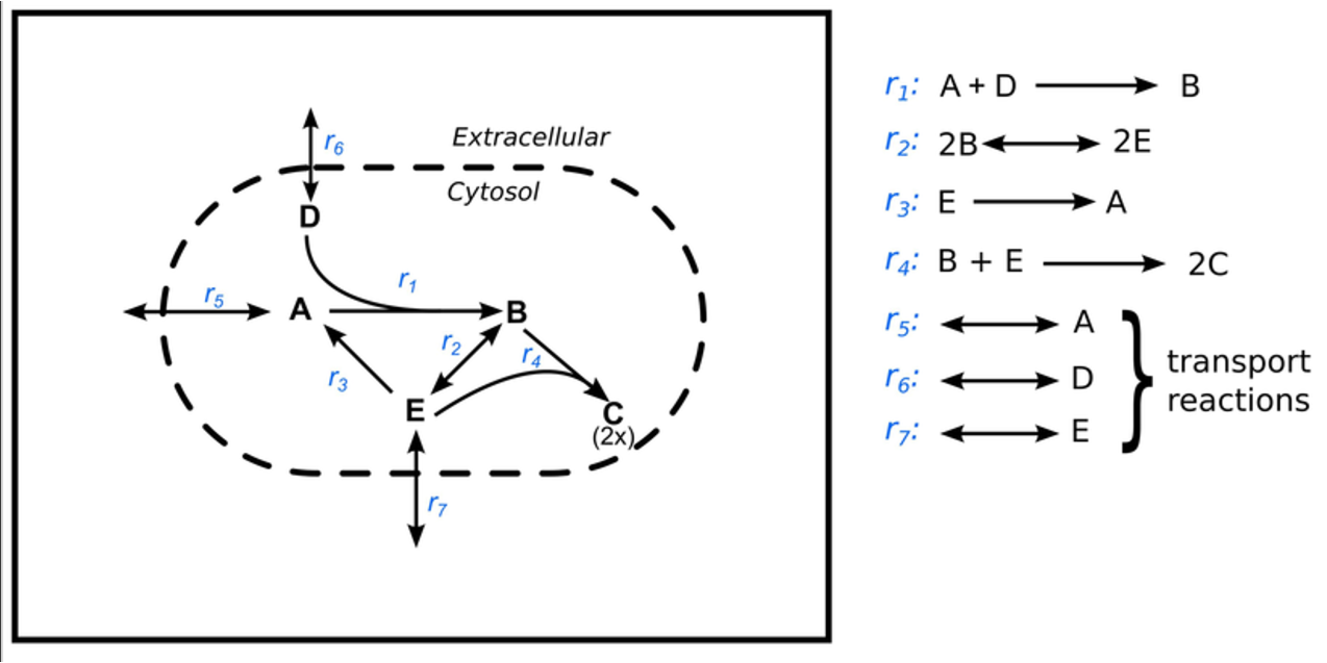
\includegraphics[width=\textwidth]{figures/mass-balance-1}
\caption{Example of metabolic network}
\end{figure}

\end{minipage}%
\begin{minipage}{0.5\textwidth}
\begin{figure}
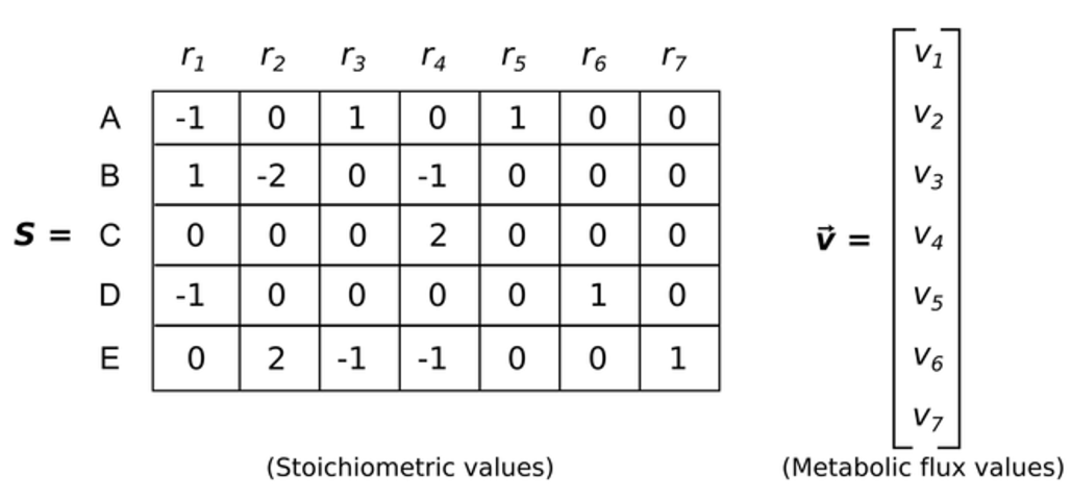
\includegraphics[width=\textwidth]{figures/mass-balance-2}
\caption{A. Stoichiometry matrix representation and the flux vector v}
\end{figure}

\end{minipage}

}

\only<3> {

\framesubtitle{Flux Balance Analysis \tiny \citep{Orth2010}}

\begin{exampleblock}{Metabolic model}
From a GEM, a model metabolic has the capacity to simulate and to predict on the metabolic content
\end{exampleblock}
\textbf{Constraint-based approaches}
\begin{minipage}{0.5\textwidth}

\begin{align*}
\begin{split}
    \text{maximiser/minimiser }\text{$f_{obj}$} \\
    \text{tel que } (S.v)_{int} = 0\\
    \text{et } \text{$v_{i_{min}}$} \leq v_i \leq \text{$v_{i_{max}}$}
\end{split}
\end{align*}

\begin{figure}
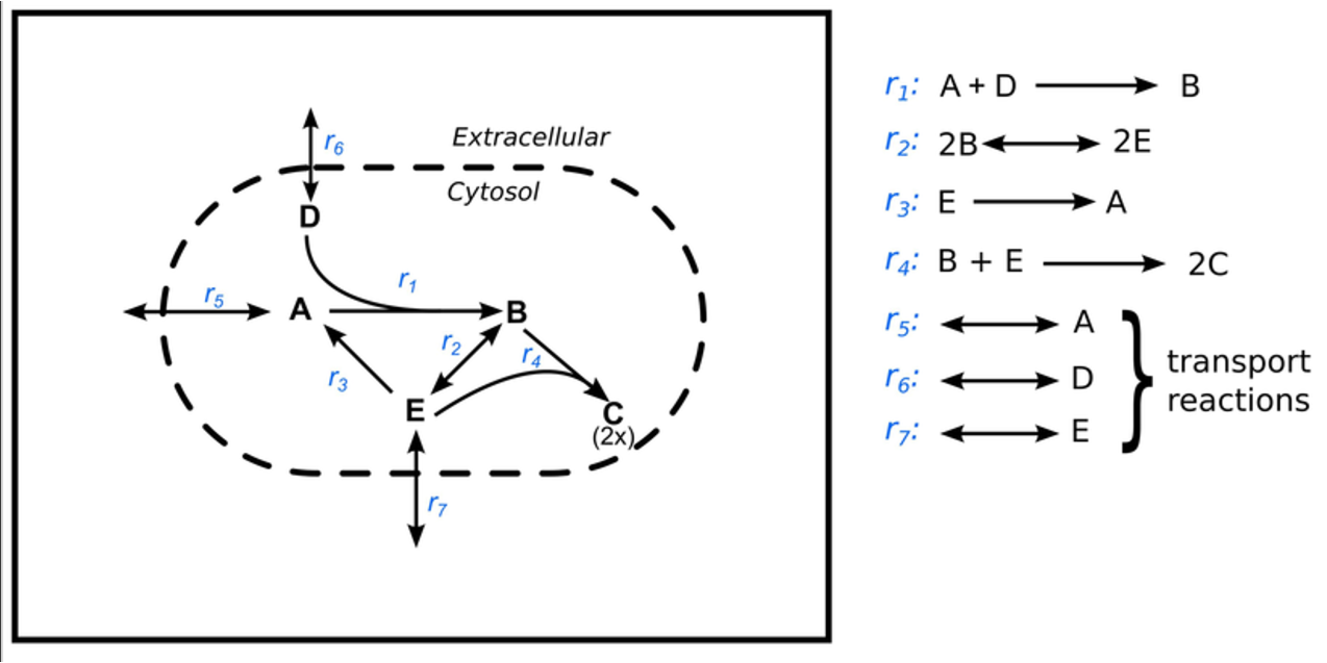
\includegraphics[width=\textwidth]{figures/mass-balance-1}
\caption{Example of metabolic network}
\end{figure}

\end{minipage}%
\begin{minipage}{0.5\textwidth}
\begin{figure}
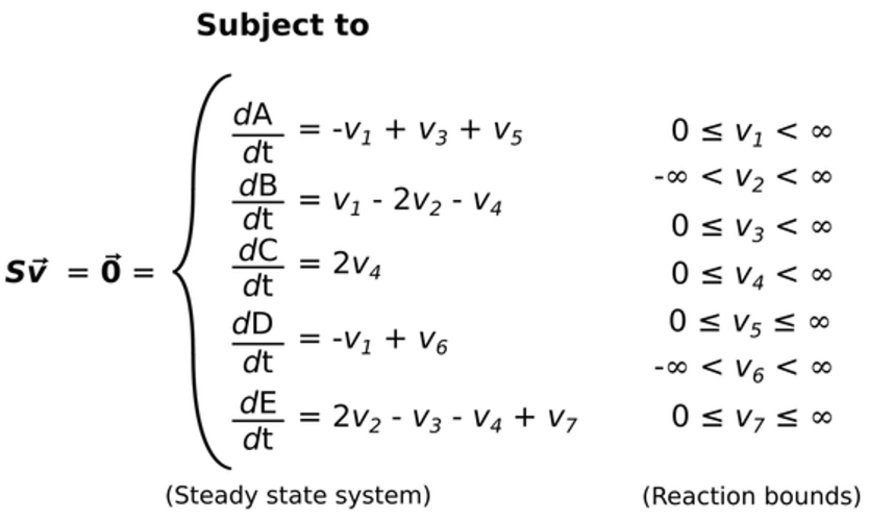
\includegraphics[width=\textwidth]{figures/mass-balance-3}
\caption{B. Linear programming problem.}
\end{figure}

\end{minipage}



}
\end{frame}

\begin{frame}
\frametitle{Flux application}
\centering
\begin{tikzpicture}
   \node (x) [circle, draw] at (0,0)   {X};
   \node (a) [circle, draw] at (2,0)   {A};
   \node (b) [circle, draw] at (4,0)   {C};
   \node (c) [circle, draw] at (3,1)   {D};
   \node (d) [circle, draw] at (5,-1)   {E};
   \node (e) [circle, draw] at (3.5,-2)   {F};
          
    \node (f) [rectangle, draw] at (1,0) {$r_1$};
  	\node (g) [rectangle, draw] at (3,0)  {$r_2$};
  	\node (h) [rectangle, draw] at (5,0)   {$r_3$};
  	\node (i) [rectangle, draw] at (4,-1)   {$r_4$};
  	\node (j) [rectangle, draw] at (5,-2)   {$r_5$};


	\draw [line width=2pt,yellow] (x) edge[->] (f);	
	\draw [line width=1.5pt,yellow](f) edge[->] (a);
		\draw [line width=0.5pt,yellow](f) edge[->] (c);
			\draw [line width=1.5pt,yellow](a) edge[->] (g);
				\draw [line width=1.5pt,yellow](g) edge[->] (b);
					\draw [line width=1.5pt,yellow](b) edge[->] (h);
						\draw [line width=0.5pt,yellow](h) edge[<-] (c);
							\draw [line width=2pt,yellow](h) edge[->] (d);
      
	\graph { (b) <- (i) <- (d) };       
	\graph { (d) <- (j) <- (e) };              
	\graph { (e) -> (i) };      
		
			     \draw [draw=black] (0.5,1.5) rectangle (5.5,-2.5);    
			     
			          \node (extracellular) [] at (6.5,1.5) {\tiny \textit{extracellular}};
     \node (intracellular) [] at (4.5,01) {\tiny \textit{intracellular}};	
\end{tikzpicture}

\begin{block}{}
	\begin{itemize}
		\item Topology and stoichiometry of metabolic goods
		\item Can explain metabolic  observations through reaction fluxes
		\item difficult to apply in larger scale
	\end{itemize}
\end{block}
\end{frame}

\begin{frame}{Contributions and objective}
\vspace{-0.3cm}
\begin{block}{Objective}
 Contribute to analyzing metabolic interactions of bacterial communities associated to two use cases: controlled and uncontrolled environment
\end{block}
\begin{figure}
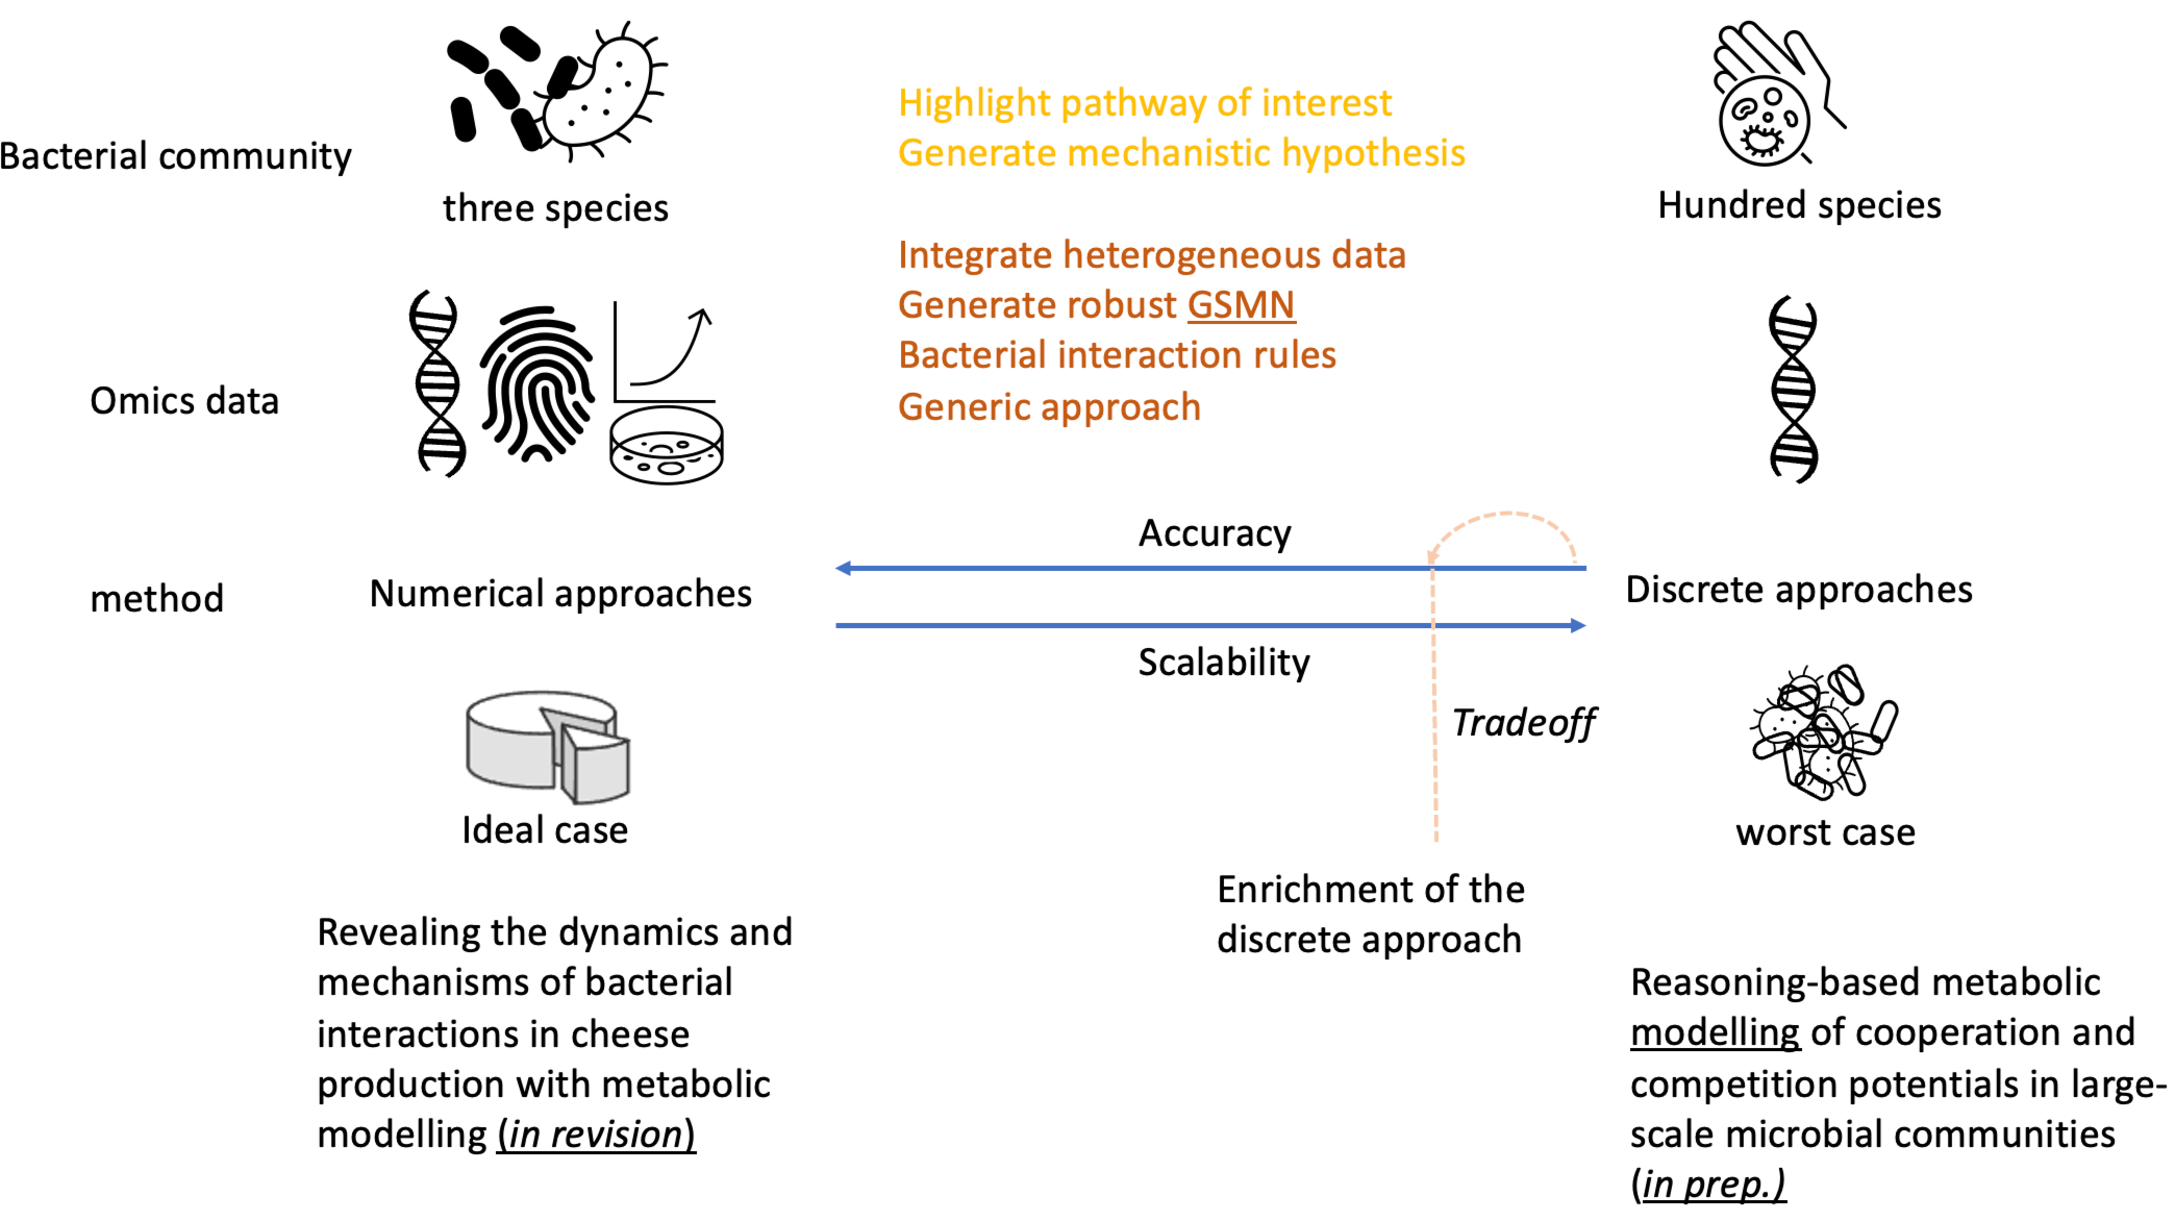
\includegraphics[width=\textwidth]{figures/objective}
\vspace{-0.6cm}\caption{Contributions in my thesis. In yellow and bown-red are respectively biological and methodological contributions}
\end{figure}


%\begin{itemize}
%\item Revealing the dynamics and mechanisms of bacterial interactions in cheese production with metabolic modelling (\textit{submitted article})
%\begin{itemize}
%\item \textcolor{blue}{Highlight pathway of interest}
%\item \textcolor{blue}{Generate mechanistic hypothesis}
%\item \textcolor{red}{Integrate heterogeneous data}
%\item \textcolor{red}{Generate robust GSMN}
%\end{itemize}
%\item Reasoning-based metabolic modelling of cooperation and competition potentials in large-scale microbial communities (\textit{in preparation})
%\begin{itemize}
%\item \textcolor{blue}{Generate mechanistic hypothesis}
%\item \textcolor{red}{Bacterial interaction rules}
%\item \textcolor{red}{Generic approach}
%\end{itemize}
%\item Enrichment of discrete models
%\begin{itemize}
%\item \textcolor{blue}{Highlight pathway}
%\item \textcolor{blue}{Generate mechanistic hypothesis}
%\item \textcolor{red}{Integrate heterogeneous constrains}
%\item \textcolor{red}{Generate logical rules}
%\end{itemize}
%
%\end{itemize}

\end{frame}

\section{Numerical model}
\begin{frame}
\frametitle{Biological context: cheese bacterial fermentation}
\begin{adjustwidth}{-0.8cm}{}
\begin{figure}
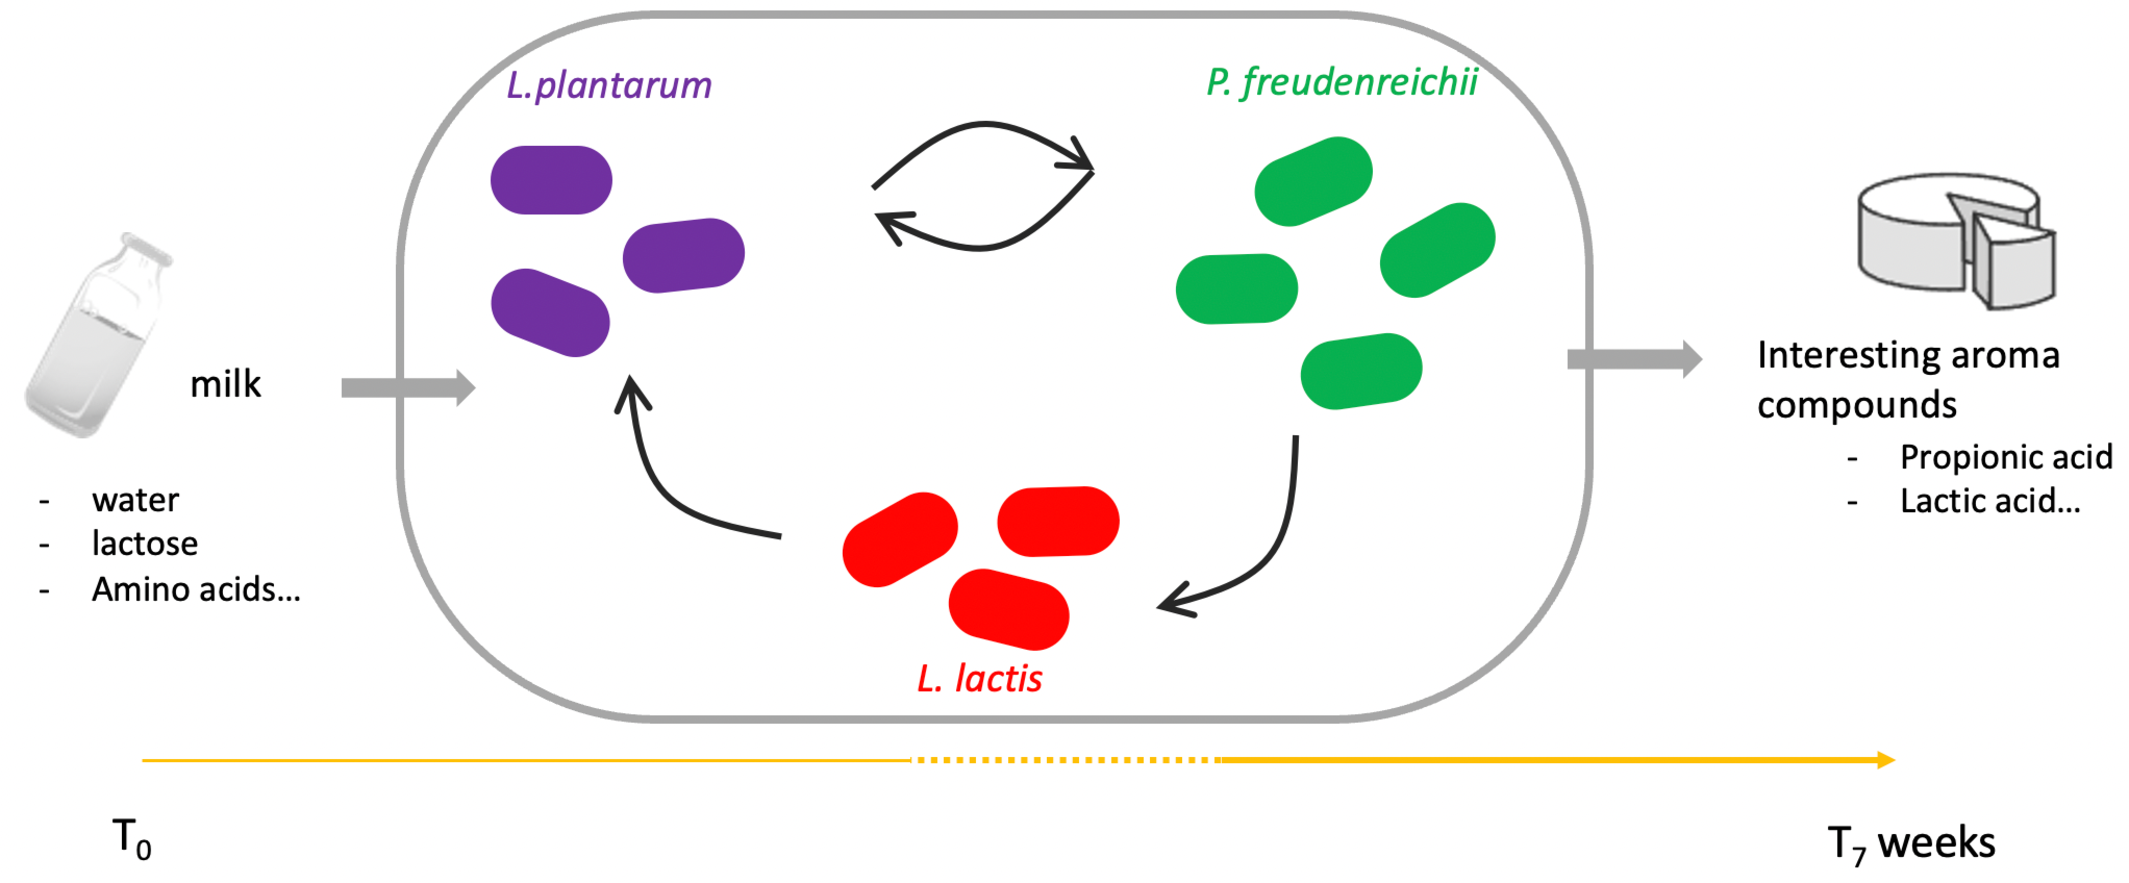
\includegraphics[width=1.15\textwidth]{figures/context-cheese}
\end{figure}
\end{adjustwidth}
\begin{block}{}
Heterogenous data are necessary for analysing bacterial fermentation
\end{block}
\end{frame}

\begin{frame}
\frametitle{Multi-omics strategy}
\begin{adjustwidth}{-0.8cm}{}
\begin{figure}
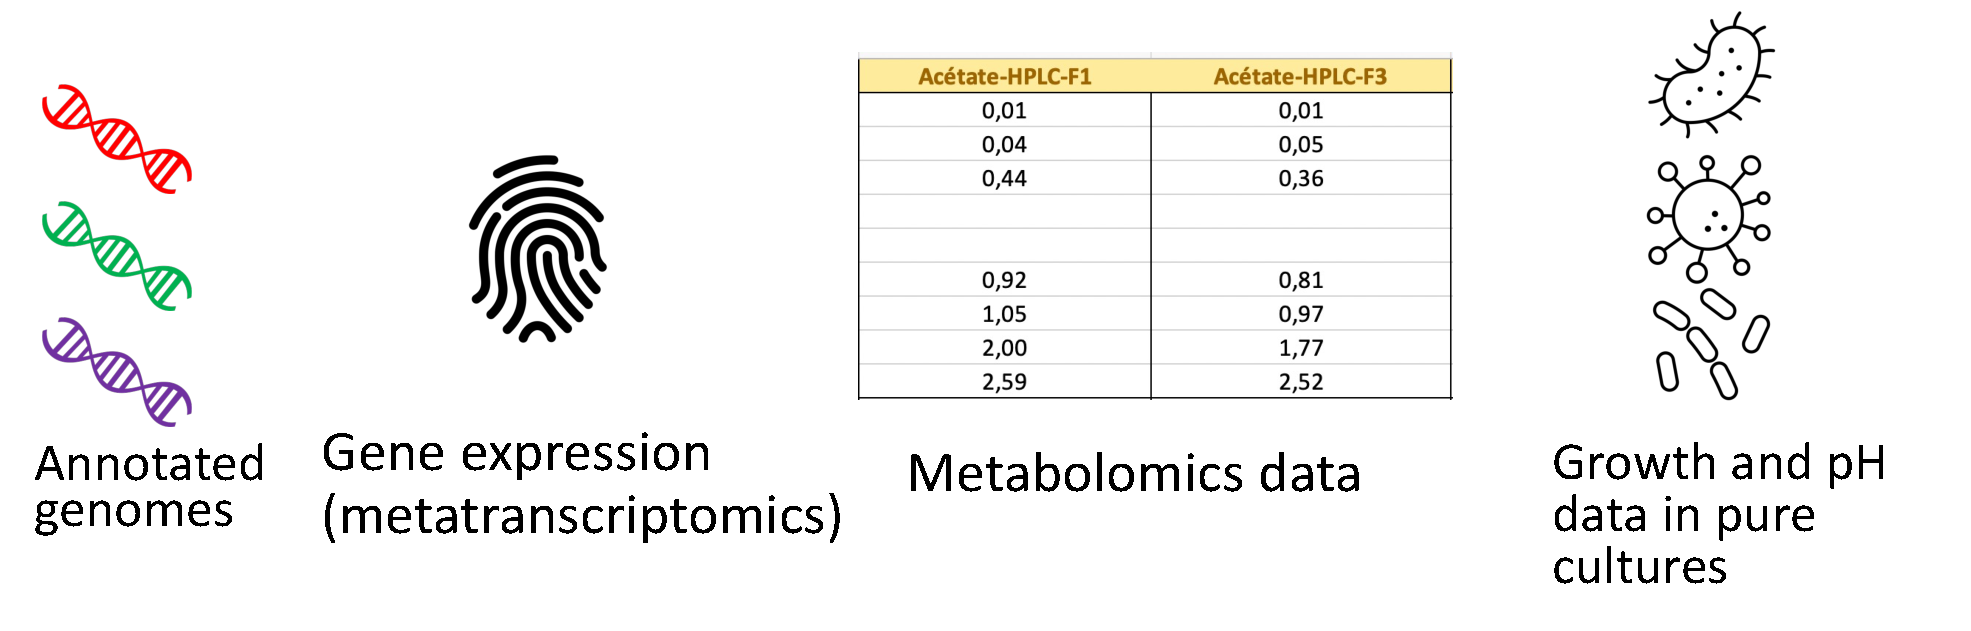
\includegraphics[width=1.15\textwidth]{figures/multi-omics}
\end{figure}
\end{adjustwidth}
\begin{block}{}
Dynamic and numerical model of the metabolism can integrate all the data
\end{block}
\end{frame}

\begin{frame}
\frametitle{Model fitting strategy}

\begin{adjustwidth}{-1cm}{}
\begin{figure}
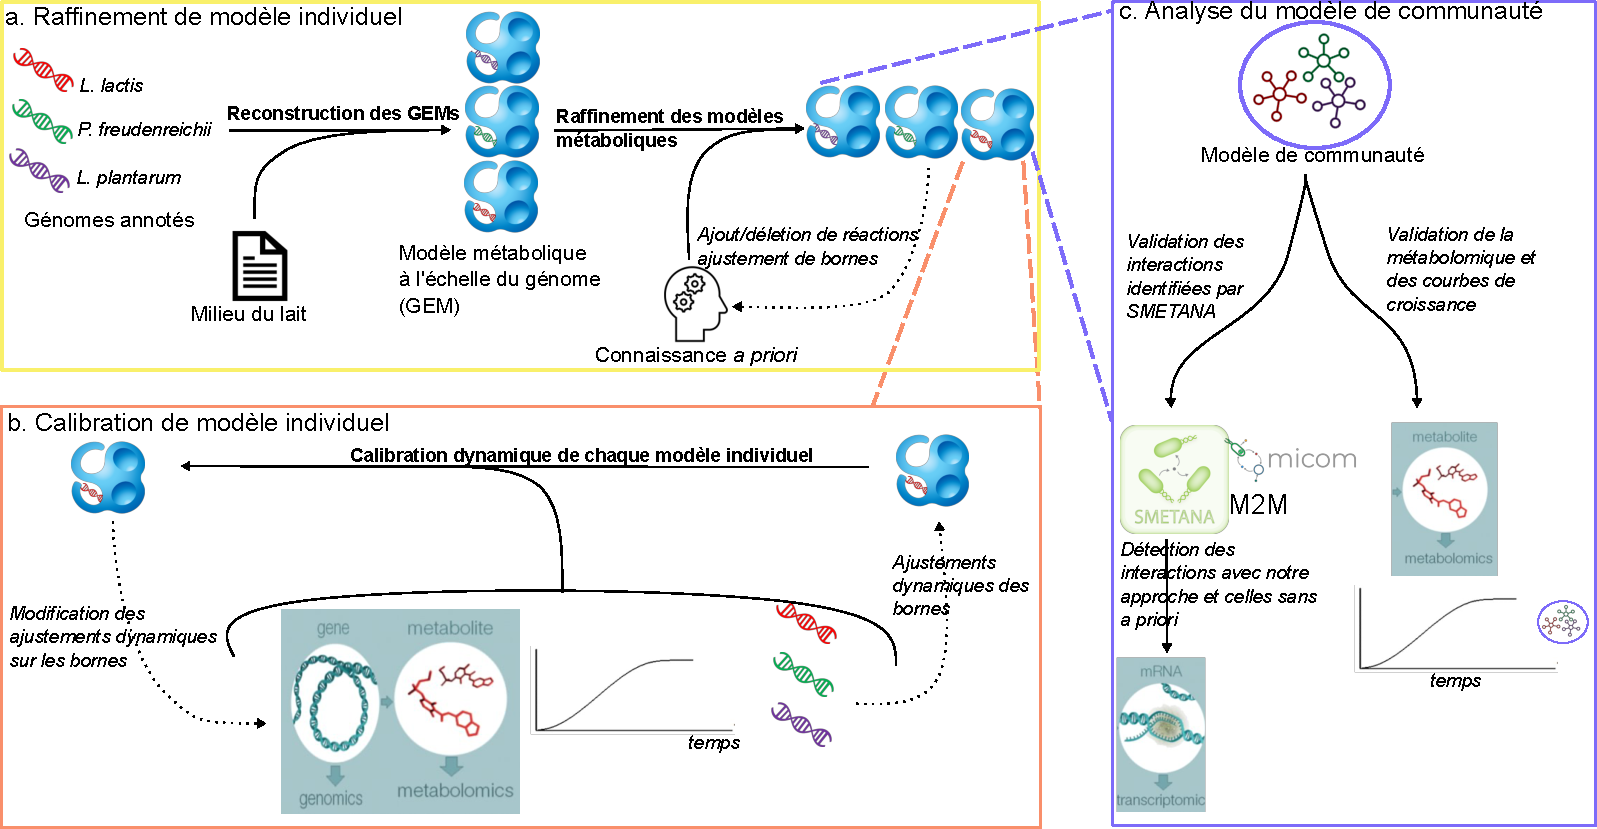
\includegraphics[width=1.2\textwidth]{figures/global.pdf}
\vspace{-0.7cm}\caption{Numerical workflow for analysing cheese bacterial fermentation}
\end{figure}
\end{adjustwidth}
\end{frame}

\begin{frame}
\frametitle{Refinement of metabolic networks - 1}

\begin{figure}
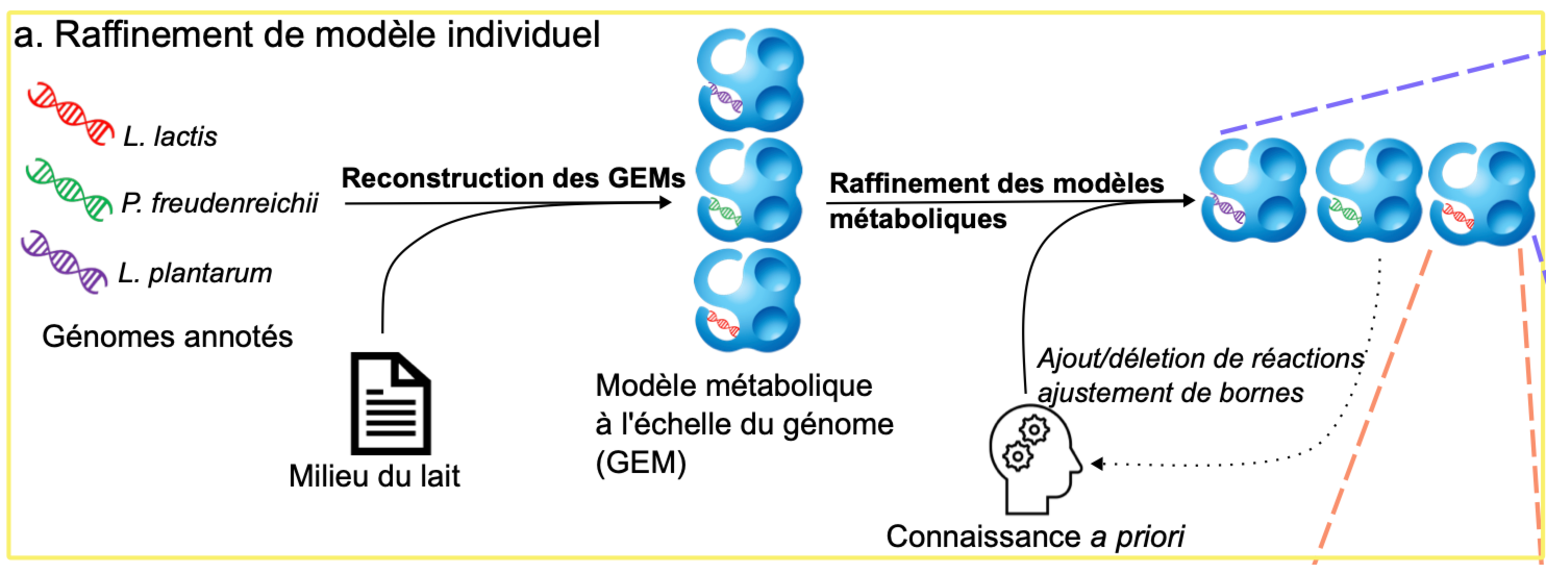
\includegraphics[width=\textwidth]{figures/global-a}
\caption{First part of the numerical workflow}
\end{figure}

\begin{block}{}
\begin{itemize}
\item Adding/removing reactions
\item Qualitative check of existing pathway and metabolic goods
\item Tedious analysis
\end{itemize}
\end{block}

\end{frame}

\begin{frame}
\frametitle{Refinement of metabolic networks - 2}
\framesubtitle{\textit{L. lactis} case}

\only<1>{
\begin{minipage}{0.7\textwidth}
\begin{adjustwidth}{-1cm}{}
\begin{figure}
\vspace{-0.1cm}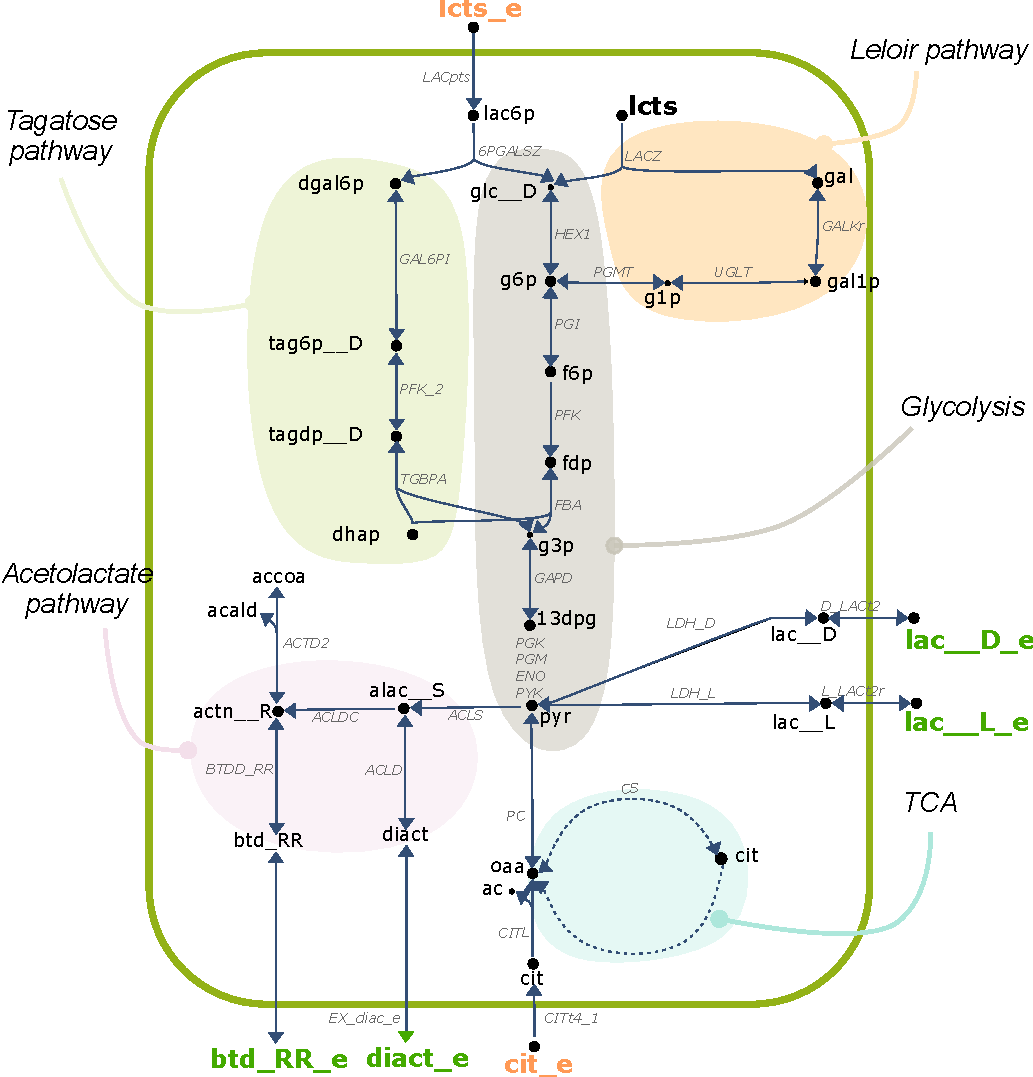
\includegraphics[width=\textwidth]{figures/carte_lactis.pdf}
\end{figure}
\end{adjustwidth}
\end{minipage}%
\begin{minipage}{0.35\textwidth}
%\begin{adjustwidth}{}{15cm}
\begin{block}{Objectif}
\begin{itemize}
\item Production of butanediol
\item activation of acetolactate pathway
\end{itemize}
\end{block}
%\end{adjustwidth}
\end{minipage}
}

\only<2>{

\begin{minipage}{0.6\textwidth}
\begin{adjustwidth}{-0.8cm}{}
\begin{figure}
\vspace{-0.1cm}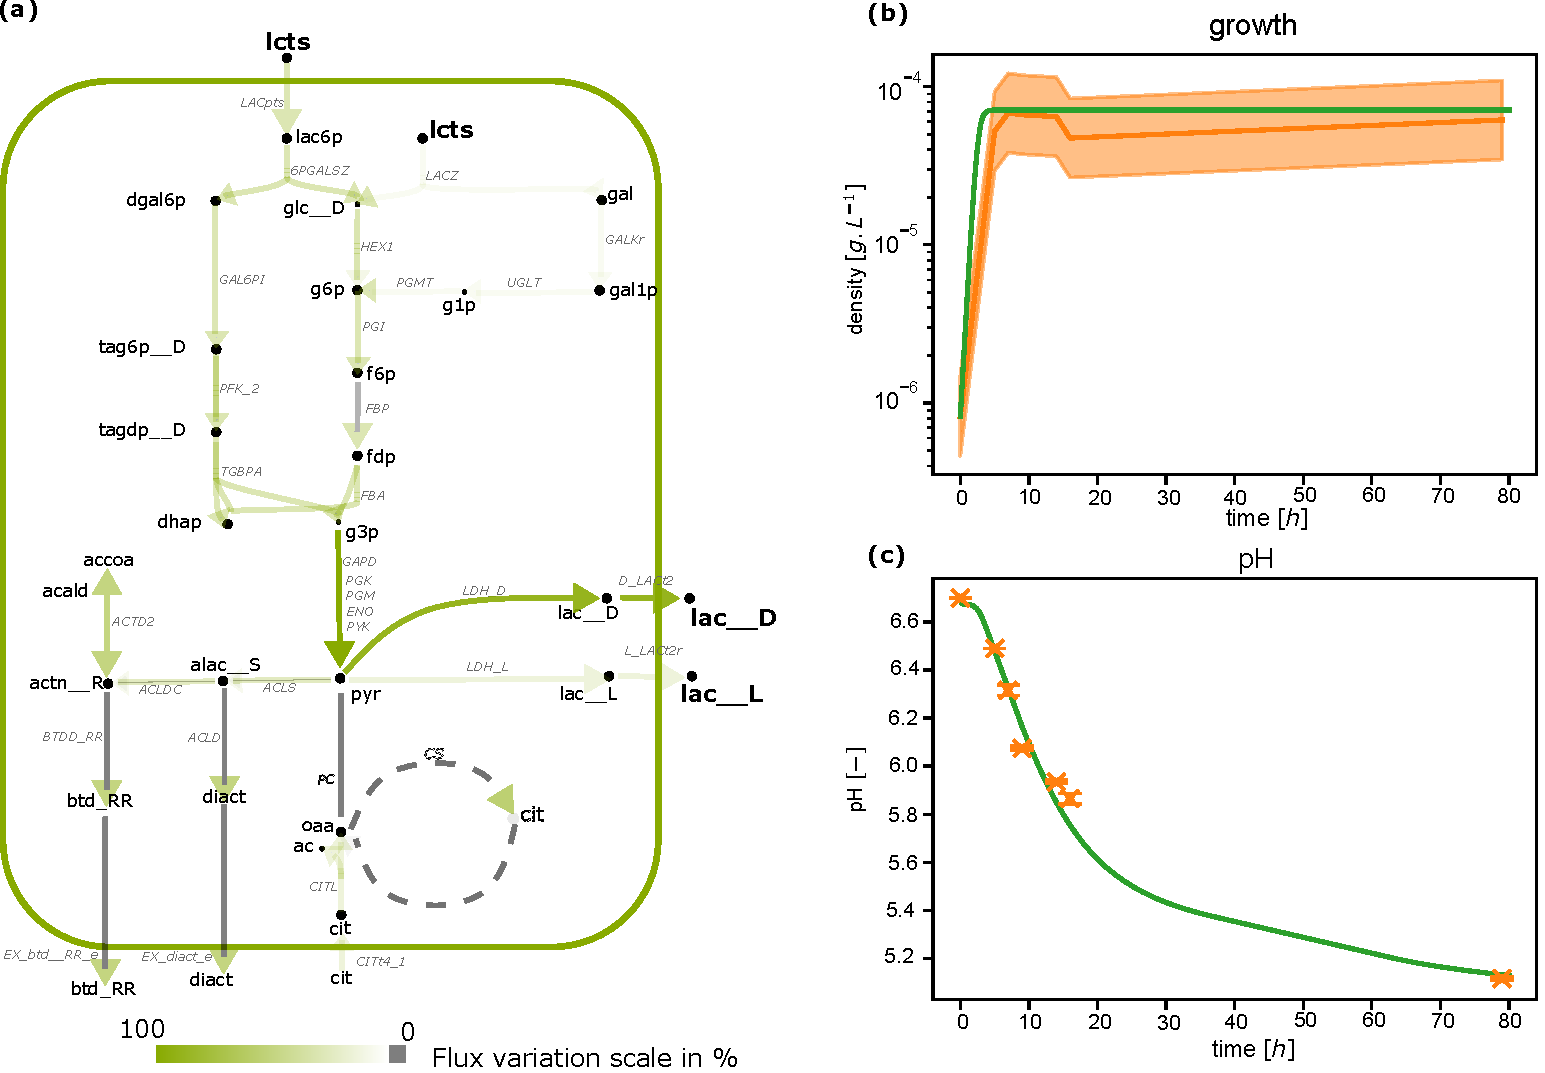
\includegraphics[width=0.95\textwidth]{figures/FIG2_opt_explo_ll.pdf}
\end{figure}
\end{adjustwidth}
\end{minipage}%
\begin{minipage}{0.45\textwidth}
\begin{block}{Objectif}
\begin{itemize}
\item Production of butanediol
\item activation of acetolactate pathway
\end{itemize}
\end{block}

\begin{block}{Refinement}
\begin{itemize}
\item Acétoine-dehydrogenase was blocked (ACTD2)
\item Modification of bounds: acétolactate decarboxylase (ACLDC) and acétolactate synthase (ACLS)
\end{itemize}
\end{block}

\end{minipage}

}
\end{frame}

\begin{frame}
\frametitle{Dynamic individual calibration}
\begin{figure}
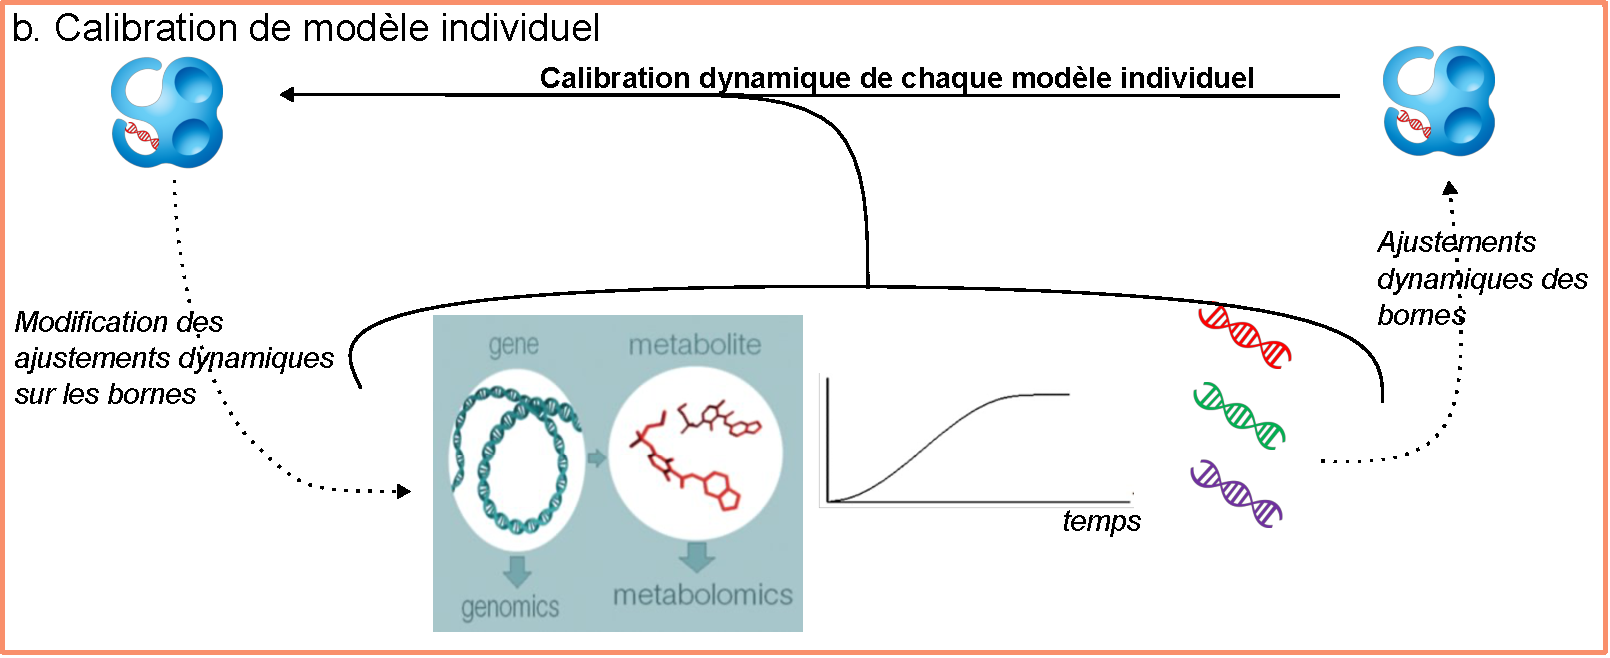
\includegraphics[width=\textwidth]{figures/calibration.pdf}
\caption{Second part of the numerical workflow}
\end{figure}

\begin{block}{}
\begin{itemize}
\item Finding optimal parameters for explaining \textbf{individual} biological observations
\item Quantitative check of metabolic goods and biomass density
\item Tedious analysis
\end{itemize}
\end{block}

\end{frame}

\begin{frame}
\frametitle{Individual metabolic model calibration}

\begin{exampleblock}{Goal}
Make individual GSMN accurate for inferring mechanistic bacterial behavior
\end{exampleblock}

\textbf{LAB} 

\begin{equation}
J(b_i,pH | \theta_i, b_{i,exp},pH_{exp} ) = \left \Vert \frac{\logten(b_i) - \logten(b_{i,exp})}{\sigma_{log,i,exp}} \right \Vert^2 + \alpha \left \Vert\frac{pH - pH_{exp}}{\sigma_{pH,exp}} \right \Vert^2 
\label{eq:optim_LAB}
\end{equation}

\textbf{\textit{P. freudenreichii}}

\begin{equation} 
J(b,m | \theta_i, b_{exp},m_{exp} ) = \left \Vert \frac{\logten(b) - \logten(b_{exp})}{\sigma_{log,b,exp}} \right \Vert ^2 + \alpha \left \Vert \frac{m - m_{exp}}{\sigma_{m,exp}} \right \Vert^2 
\label{eq:optim_freud}
\end{equation}

\begin{block}{Data}
\begin{itemize}
\item Metabolomics
\item Growth and pH in pure cultures
\end{itemize}
\end{block}

\end{frame}


\begin{frame}
\frametitle{Bacterial fermentation: a dynamic process}

\begin{adjustwidth}{-0.8cm}{}
\begin{figure}

\includegraphics[width=1.15\textwidth]{figures/tango}
\end{figure}
\end{adjustwidth}

\begin{block}{Challenge}
\begin{itemize}
\item Nutrient concentration over time
\item The dynamic of bacterial density
\item Resource sharing 
\end{itemize}
\end{block}

\begin{block}{Solution}
\begin{itemize}
\item Compute dynamic model of the metabolism (dFBA) \tiny \citep{Mahadevan.2002}
\end{itemize}
\end{block}
\end{frame}

\begin{frame}
\frametitle{Dynamic modeling of the metabolism (dFBA)}

\only<1>{
\framesubtitle{Compute the total flux}

\begin{figure}[t]
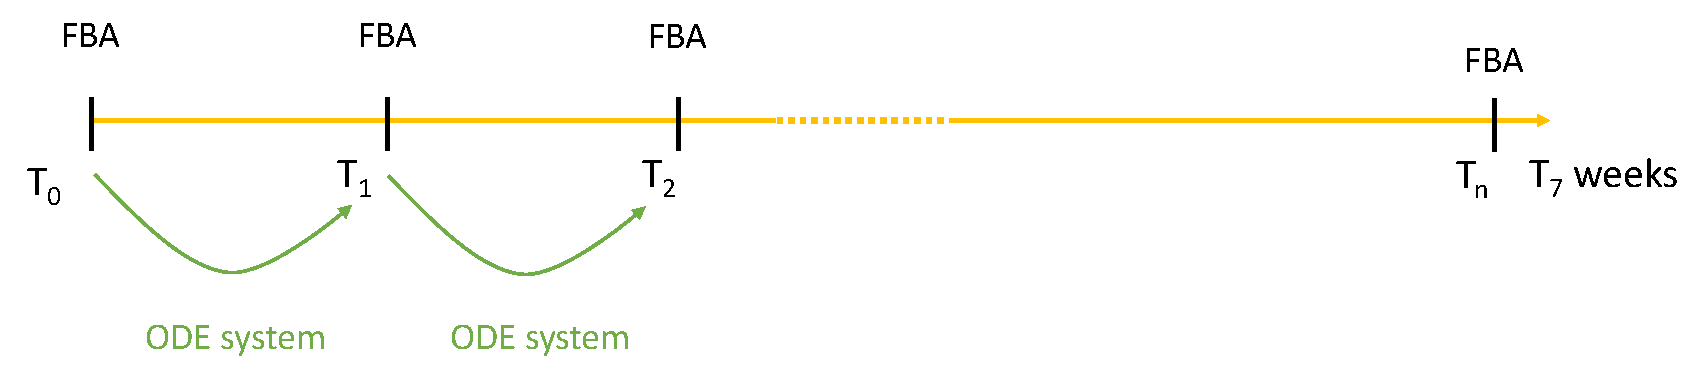
\includegraphics[width=\textwidth]{figures/time-dfba.pdf}
\end{figure}
\begin{align}
\hspace{-2cm}
F_j & =\sum_{i \in \mathcal{B}} {\mu}_{i,j}\left((c^{ex}_{min,i},c^{ex}_{max,i})(b^n,m^n)\right) b_i 
\end{align} 
$F_j$ total flux computed in $mmol.gDW^{-1}.h^{-1}$\\
${\mu}_{i,j}\left((c^{ex}_{min,i},c^{ex}_{max,i})(b^n,m^n)\right) b_i$ is the correspondence between exchange reaction, bacterial and metabolite constraints in the system  from a given environment.
}

\only<2>{
\framesubtitle{Compute bacteria \textbf{densities} and metabolites \textbf{concentrations}}
\begin{figure}[t]
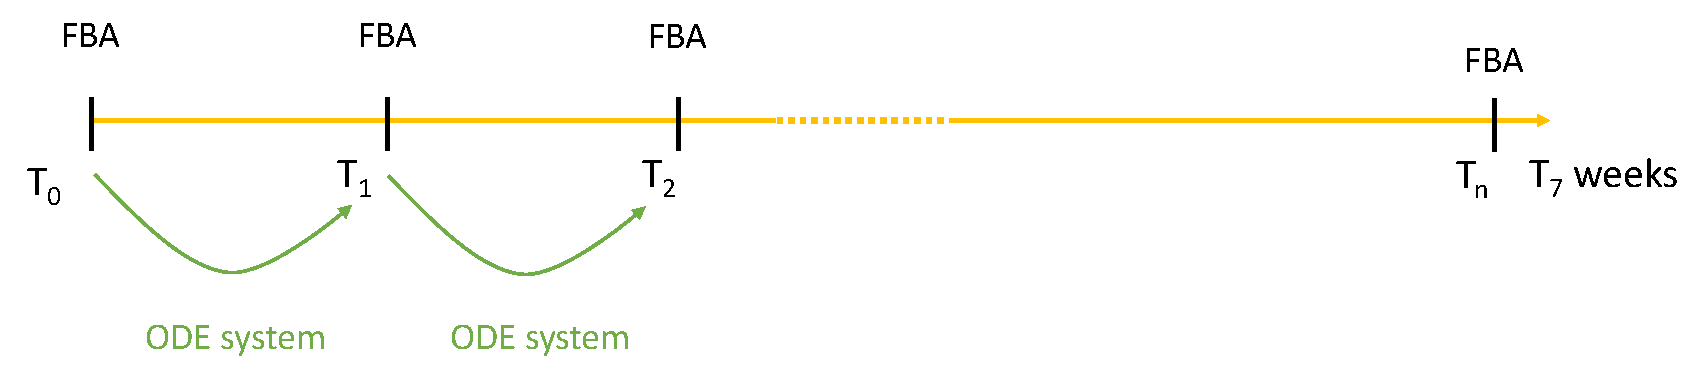
\includegraphics[width=\textwidth]{figures/time-dfba.pdf}
\end{figure}
\begin{align}
\hspace{-2cm}
F_j & =\sum_{i \in \mathcal{B}} {\mu}_{i,j}\left((c^{ex}_{min,i},c^{ex}_{max,i})(b^n,m^n)\right) b_i \\
\hspace{-2cm}
b_i^{n+1}& = b_i^n+\Delta t* F_{b_i} \\
\hspace{-2cm}
m_j^{n+1}& = \begin{cases} m_i^n+\Delta t* F_{j} & \text{ si } F_j>0 \text{ (cas explicite)}\\
m_j^n/(1-\Delta t * F_j/m_j^n) & \text{ sinon (cas implicite)}
\end{cases}
\end{align}

\begin{block}{}
Euler semi implicit schema guarantees the positivity of the solution
\end{block}
}

\only<3>{

\framesubtitle{General dynamic model}
\begin{figure}[t]
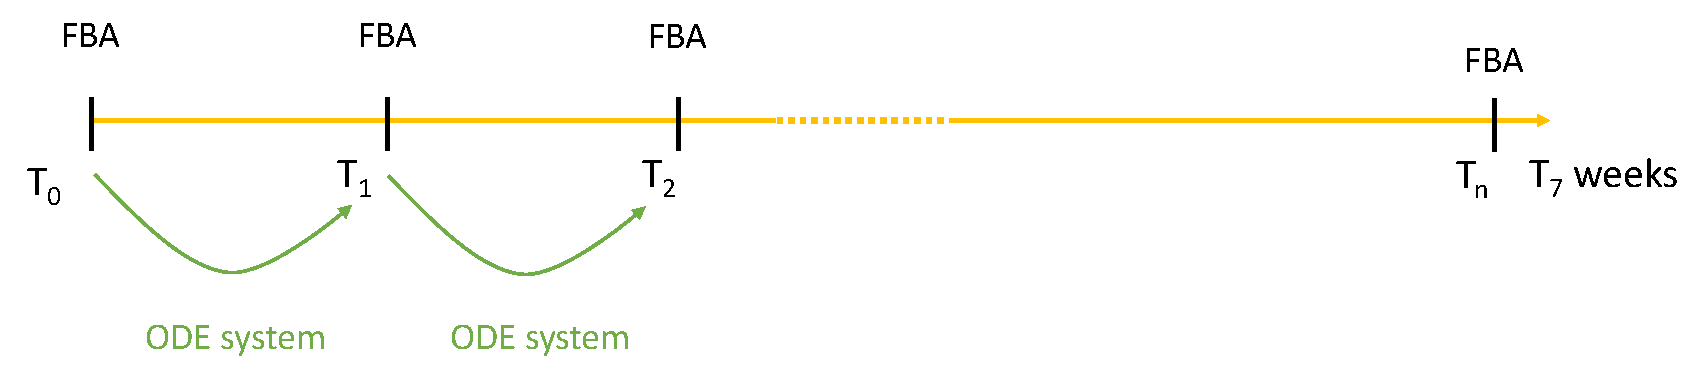
\includegraphics[width=\textwidth]{figures/time-dfba.pdf}
\end{figure}
\begin{align}
\hspace{-2cm}
F_j & =\sum_{i \in \mathcal{B}} {\mu}_{i,j}\left((c^{ex}_{min,i},c^{ex}_{max,i})(b^n,m^n)\right) b_i \\
\hspace{-2cm}
b_i^{n+1}& = b_i^n+\Delta t* F_{b_i} \\
\hspace{-2cm}
m_j^{n+1}& = \begin{cases} m_i^n+\Delta t* F_{j} & \text{ si } F_j>0 \text{ (cas explicite)}\\
m_j^n/(1-\Delta t * F_j/m_j^n) & \text{ sinon (cas implicite)}
\end{cases}\\
\hspace{-2cm}
    \partial_t b_i& = \mathcal{R}_{i}(b_i) {\mu}_{i,i}\left((c^{ex}_{min,i},c^{ex}_{max,i})(b,m)\right) b_i  \\
    \hspace{-2cm}
    \partial_t m_j &= \sum_{i \in \mathcal{B}} {\mu}_{i,j}\left((c^{ex}_{min,i},c^{ex}_{max,i})(b,m)\right) b_i 
\end{align}

\begin{block}{}
Bacterial densities and metabolites concentrations are therefore computed in $g.L^{-1}$ and $mmol.L{-1}$ 
\end{block}
}
\end{frame}

\begin{frame}
\frametitle{Dynamic modulations}

\textbf{Usual consumption limitation}
\begin{equation}
c^{ex}_{min,i,j} = max(-\frac{m_{lcts_e}}{\Delta t*\sum_{i \in \mathcal{M_j}} b_i}, v^{int}_{i,j})
\end{equation}

\begin{block}{}
\begin{itemize}
\item $\mathcal{M_j}$ Bacteria subset can metabolize $_j$
\item Balanced resource sharing 
\end{itemize}

\end{block}

\textbf{Lactose consumption}
\begin{equation}
c^{ex}_{min,i,j} = max(-\frac{m_{lcts_e}}{\Delta t*\sum_{i \in \mathcal{M}(lcts_e)} b_i},-\mu_{max,lcts}*10^{(-k_{lac}*\phi_{undiss})}-\mu_{min,lcts})
\end{equation}
\begin{block}{}
\begin{itemize}
\item Lactose consumption negatively regulated by the non dissociated form of acid lactic
\end{itemize}
\end{block}


\textbf{pH regulation}


\begin{equation}
\phi_{undiss}(m_{lac\_\_L\_e},m_{lac\_\_D\_e}) = \frac{m_{lac\_\_L\_e}+m_{lac\_\_D\_e}}{1+ 10^{c_1 * (m_{lac\_\_L\_e}+m_{lac\_\_D\_e})+c_2}}.
\label{eq:undissociated-lactate}
\end{equation}

\begin{block}{}
\begin{itemize}
\item approximation of pH - pKa
\end{itemize}
\end{block}
\end{frame}


\begin{frame}
\frametitle{Model validation}

\only<1>{
\framesubtitle{\textit{L. plantarum}}
\begin{adjustwidth}{-0.6cm}{}
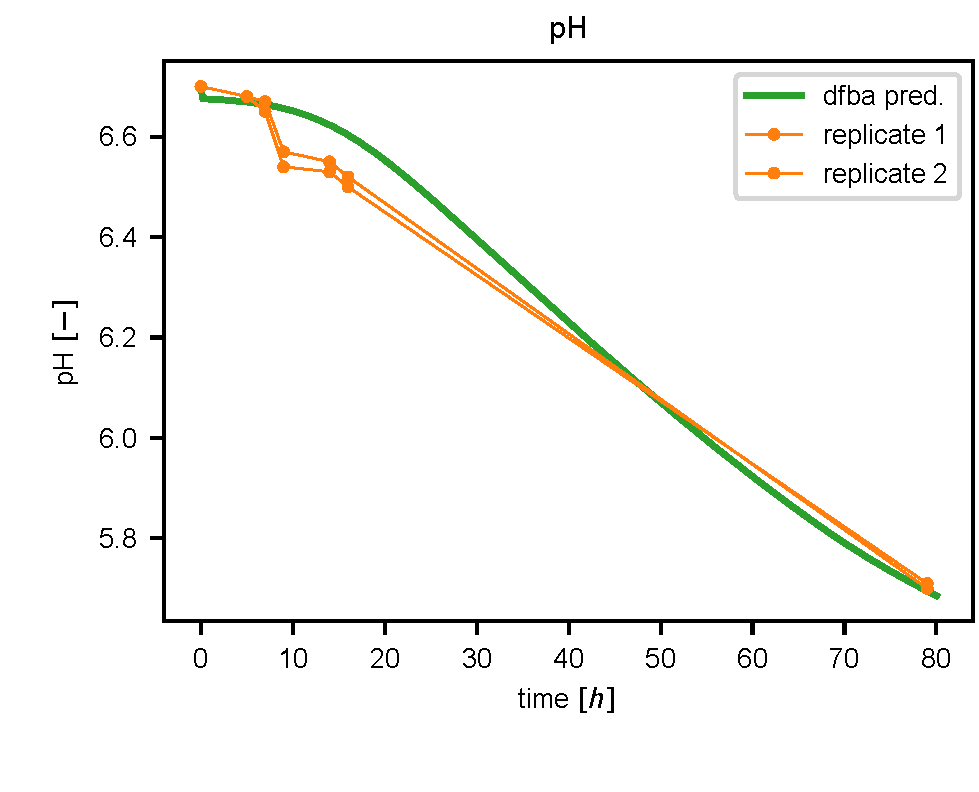
\includegraphics[width=1.1\textwidth]{figures/validation-lp.pdf}
\end{adjustwidth}
\begin{block}{}
Dynamic model of \textit{L. plantarum} explains its experimental growth and pH
\end{block}
}


\only<2>{
\framesubtitle{\textit{L. lactis}}
\begin{adjustwidth}{-0.6cm}{}
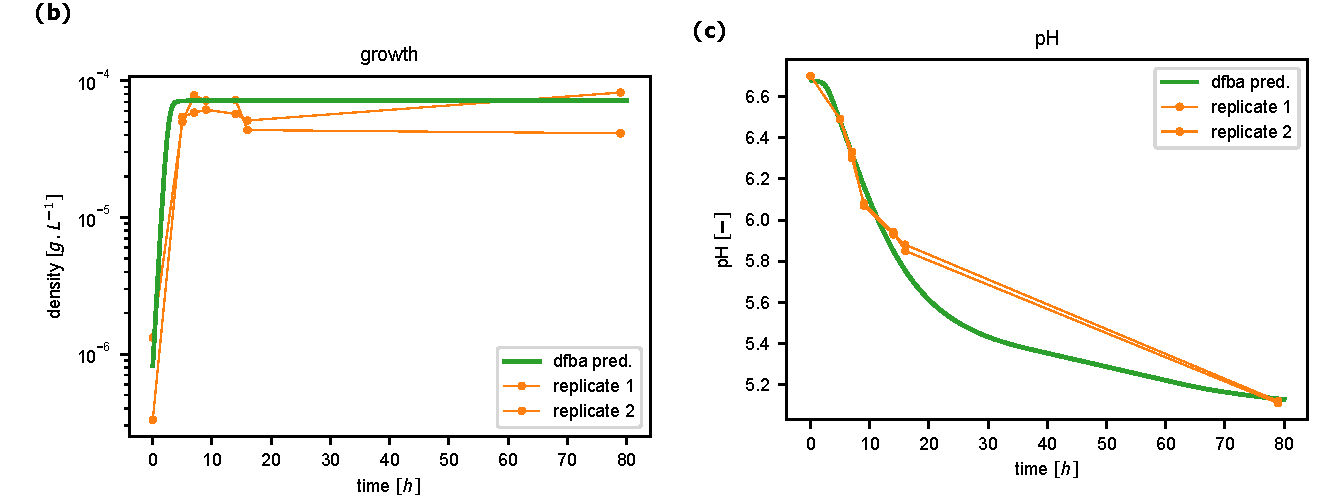
\includegraphics[width=1.1\textwidth]{figures/validation-ll.pdf}
\end{adjustwidth}
\begin{block}{}
Dynamic model of \textit{L. lactis} explains its experimental growth and pH
\end{block}
}


\only<3>{
\framesubtitle{\textit{P. freudenreichii}}
\begin{adjustwidth}{-0.6cm}{}
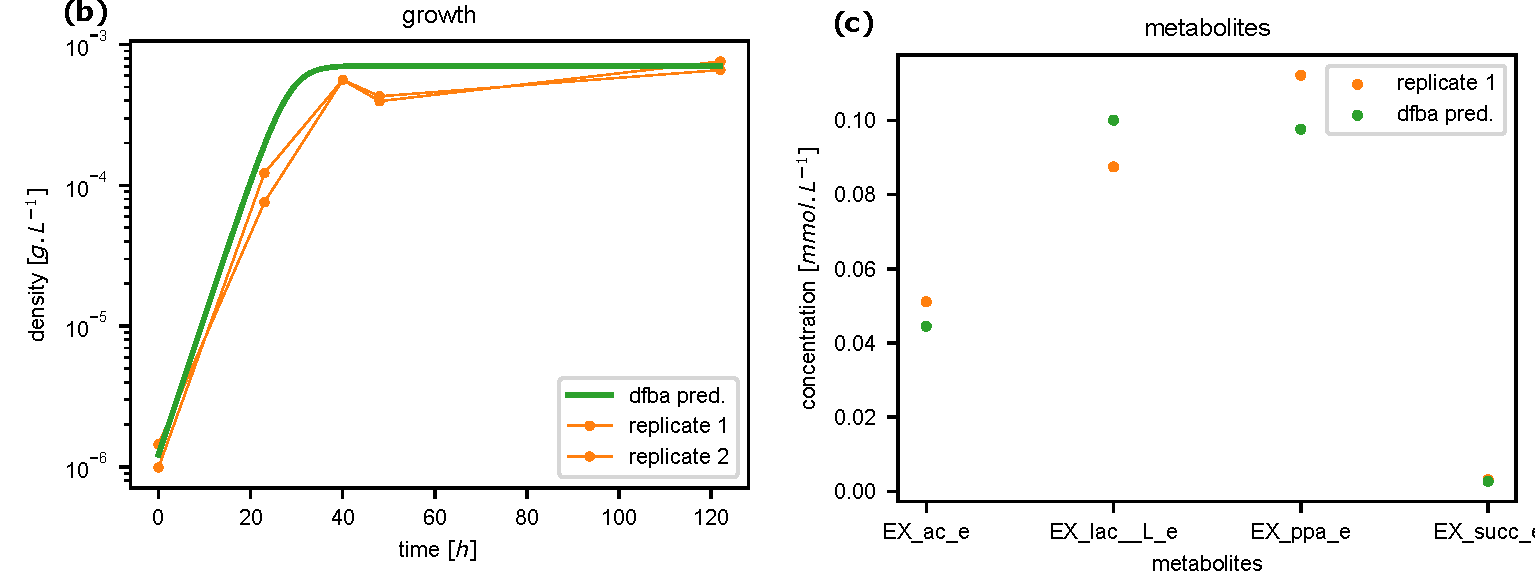
\includegraphics[width=1.1\textwidth]{figures/validation-pf.pdf}
\end{adjustwidth}
\begin{block}{}
Dynamic model of \textit{P. freudenreichii} explains its experimental growth and acid dosages
\end{block}

}

\begin{block}{home message}
Individual metabolic model well calibrated $\rightarrow$ retrieve experimental data
\end{block}

\end{frame}

\begin{frame}
\frametitle{Community validation}

\begin{figure}
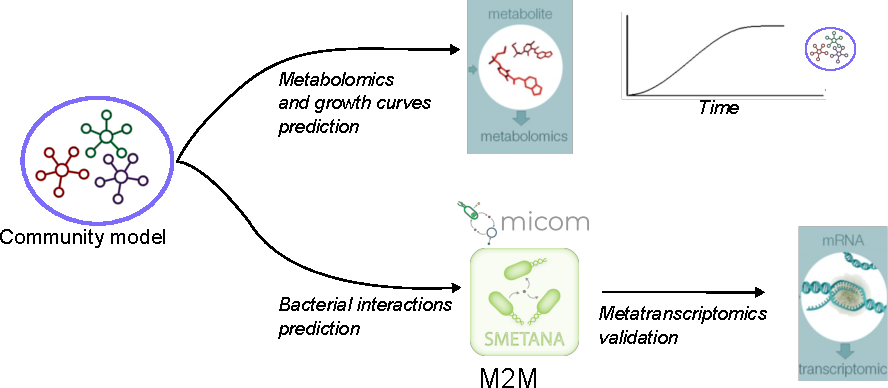
\includegraphics[width=\textwidth]{figures/com-validation.pdf}
\end{figure}
\begin{block}{}
\begin{itemize}
\item Bacterial interaction \textbf{prediction}
\item Metabolic explanation of biological observations
\item \textbf{No community calibration}
\end{itemize}
\end{block}
\end{frame}

\begin{frame}
\frametitle{Community prediction}
\framesubtitle{Growth and pH}

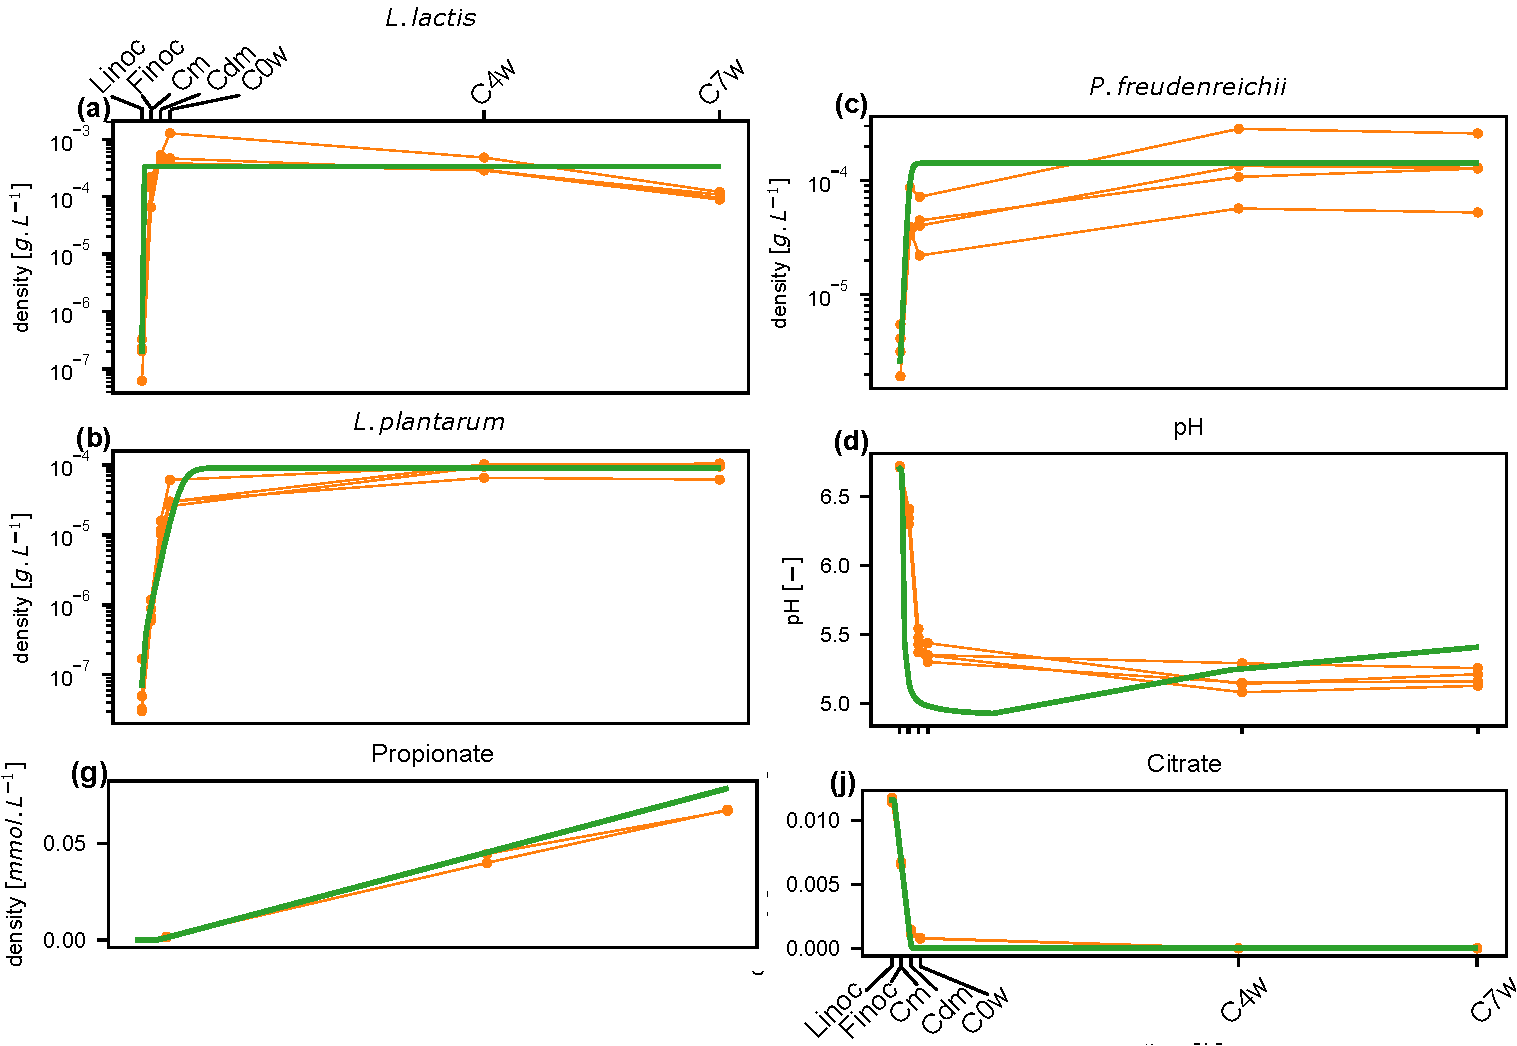
\includegraphics[width=\textwidth]{figures/community-pred-growth.pdf}
\begin{block}{}
\begin{itemize}
\item Growth well predicted for all bacteria
\item Lactate proxy production can explain the observed pH
\end{itemize}
\end{block}
\end{frame}

\begin{frame}
\frametitle{Community prediction}
\framesubtitle{Metabolomics}
\begin{adjustwidth}{-0.6cm}{}
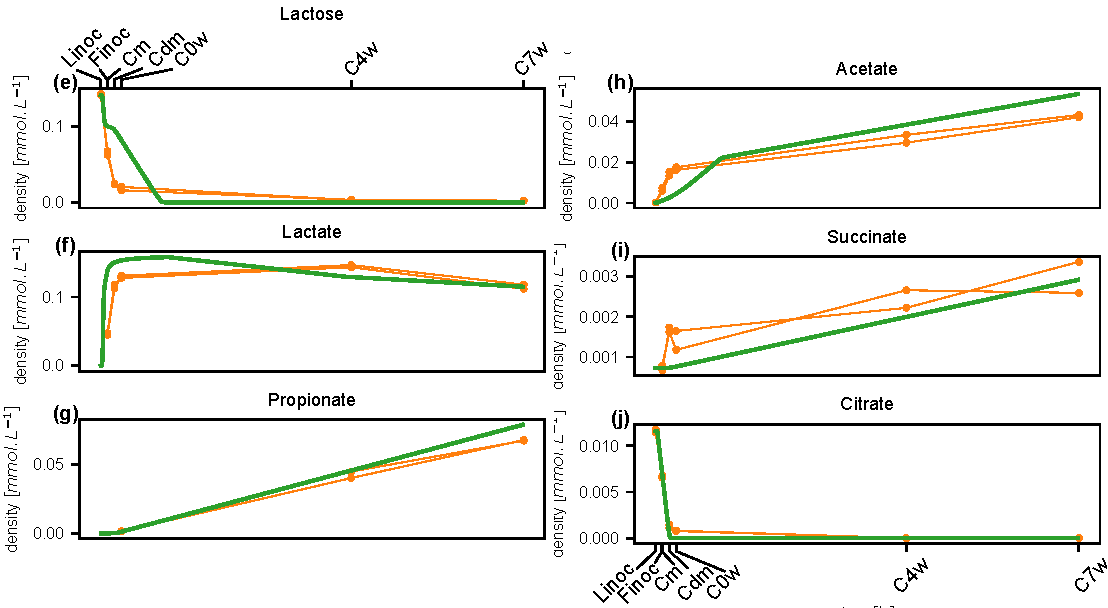
\includegraphics[width=1.1\textwidth]{figures/community-pred-metabolo.pdf}
\end{adjustwidth}
\begin{block}{}
\begin{itemize}
\item Metabolomic is well predicted 
\end{itemize}
\end{block}
\end{frame}


\begin{frame}
\frametitle{So what....}
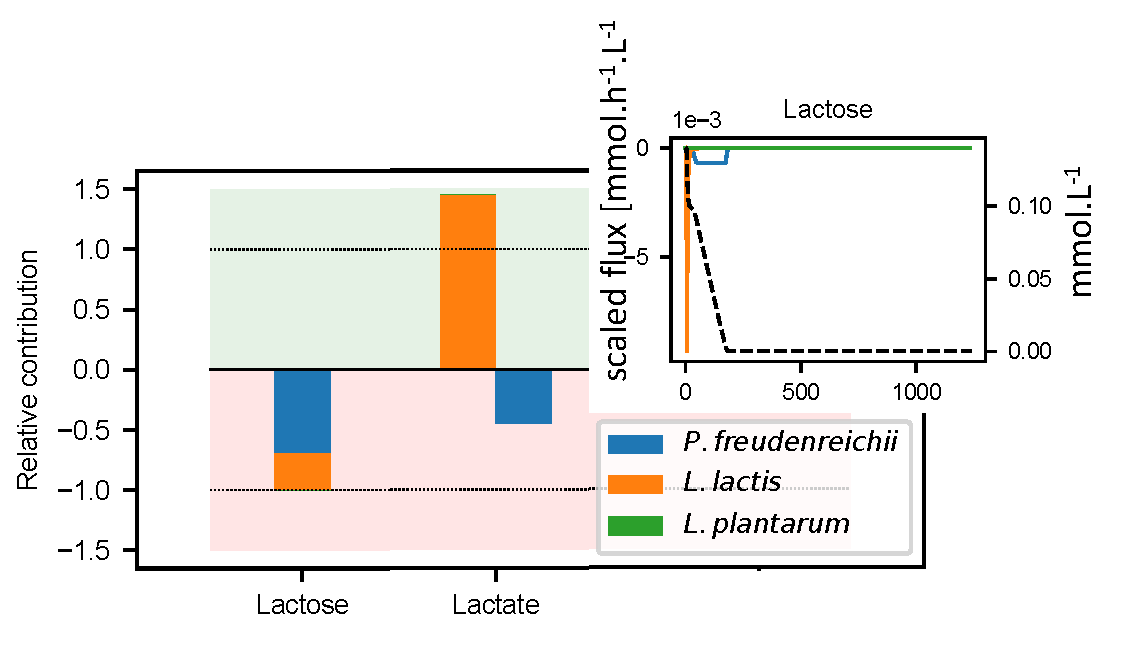
\includegraphics[width=\textwidth]{figures/relative-contribution.pdf}
\begin{minipage}{0.5\textwidth}
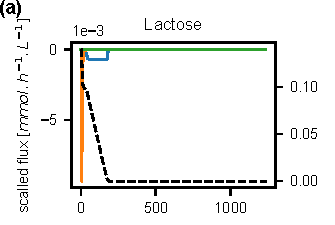
\includegraphics[width=\textwidth]{figures/lactose.pdf}
\end{minipage}%
\begin{minipage}{0.5\textwidth}
\begin{itemize}
\item 11 shared metabolites predicted with SMETANA, MiCOM (phénylalanine, succinate, xanthine..)
\item H$_2$S, ribose and glycerol seams to be relevant
\end{itemize}
\end{minipage}

\begin{itemize}
\item No competition for lactose
\item \textit{L. lactis} main lactate producer 
\item \textit{P. freudenreichii} main producer of Acetate
\end{itemize}
\end{frame}


\begin{frame}
\frametitle{Added-value and limitations}
\centering
\textbf{\huge Take home message}

\begin{minipage}{0.45\textwidth}
\begin{block}{Originality}
\begin{itemize}
\item High quality of refinement and well calibrated individual GSMN from cheese %
\item Accurate dynamic model with few optimized parameters %
\item No need of community calibration to predict community behavior %
\end{itemize}
\end{block} %
\end{minipage}\hfill
\hspace{0.5cm}
\hfill
\begin{minipage}{0.45\textwidth}
\begin{block}{Scalability issue}
\begin{itemize}
\item Refinement process is time consuming
\item The iterative methodology assume well documented GSMNs in literature
\item Based on \textit{a priori} knowledge for screening compounds
\end{itemize}
\end{block}
\end{minipage}

\begin{block}{Solution}
For screening large community, use of different formalism is required
\end{block}


\end{frame}



\section{Discrete model}

\begin{frame}
\frametitle{Discrete modelling able to screen large community}
\begin{figure}
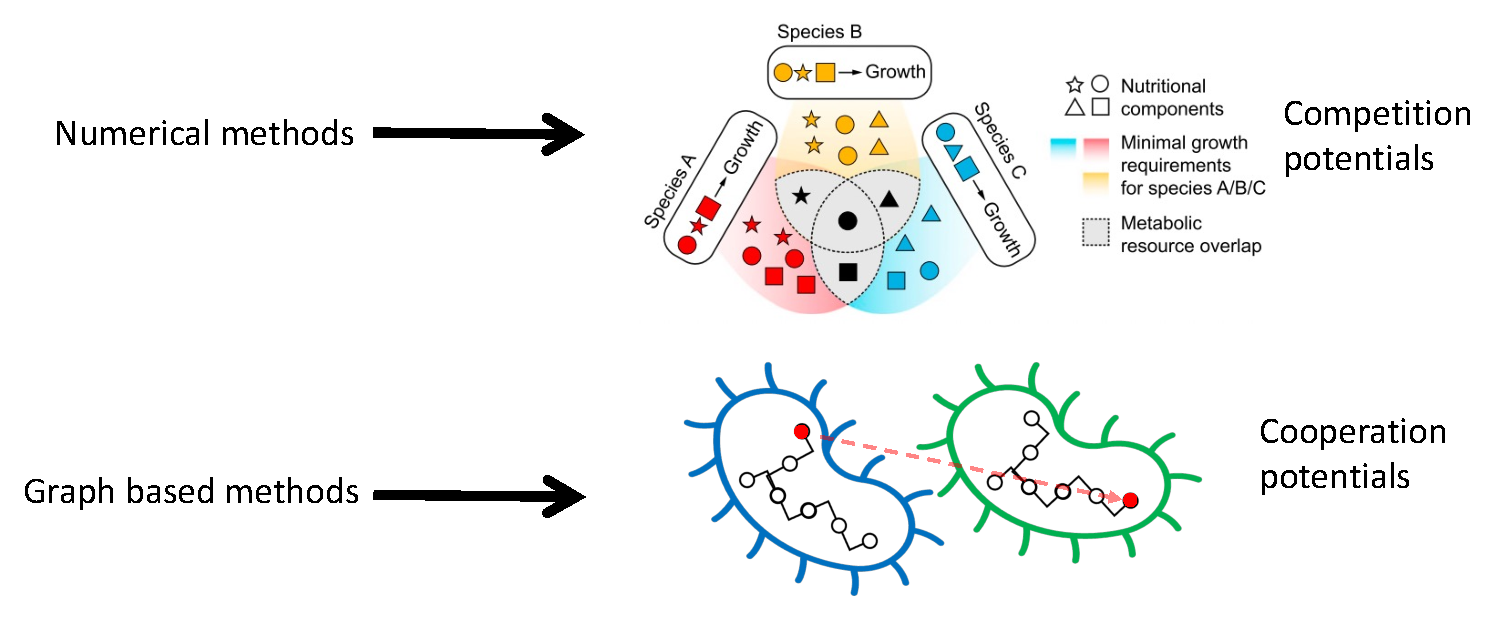
\includegraphics[width=\textwidth]{figures/sota-discrete.pdf}
\end{figure}
\begin{block}{}
\begin{itemize}
\item Competition and cooperation potential are used for describing ecosystems
\item Community size analysis up to 18 \tiny \citep{Zelezniak2015} \normalsize in a reasonable time 
\item tedious pairwise analysis for graph base methods
\item Discrete-based methods not limited by the size of community
\end{itemize}
\end{block}
\end{frame}

\begin{frame}
\frametitle{Contributions 2: Discrete approach for characterizing large-scale bacterial}
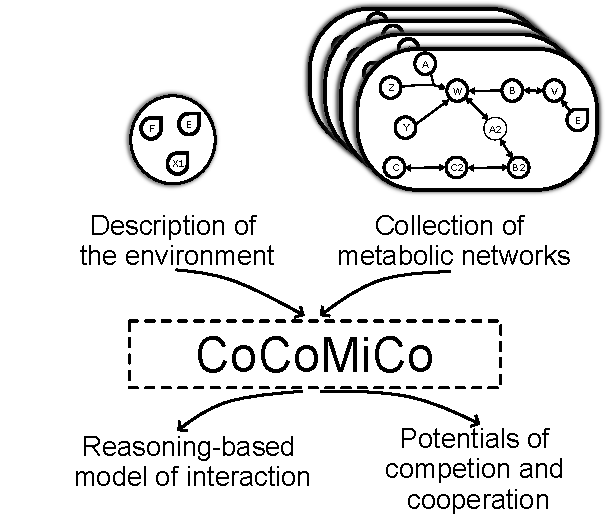
\includegraphics[width=\textwidth]{figures/concept.pdf}
\begin{block}{}
\begin{itemize}
\item Combination of the extension of network expansion algorithm and answer set programming for the calculation of cooperation and competition potentials
\item How to define cooperation and competition potentials ?
\end{itemize}
\end{block}
\end{frame}

\begin{frame}
\frametitle{Cooperation \& competition properties}
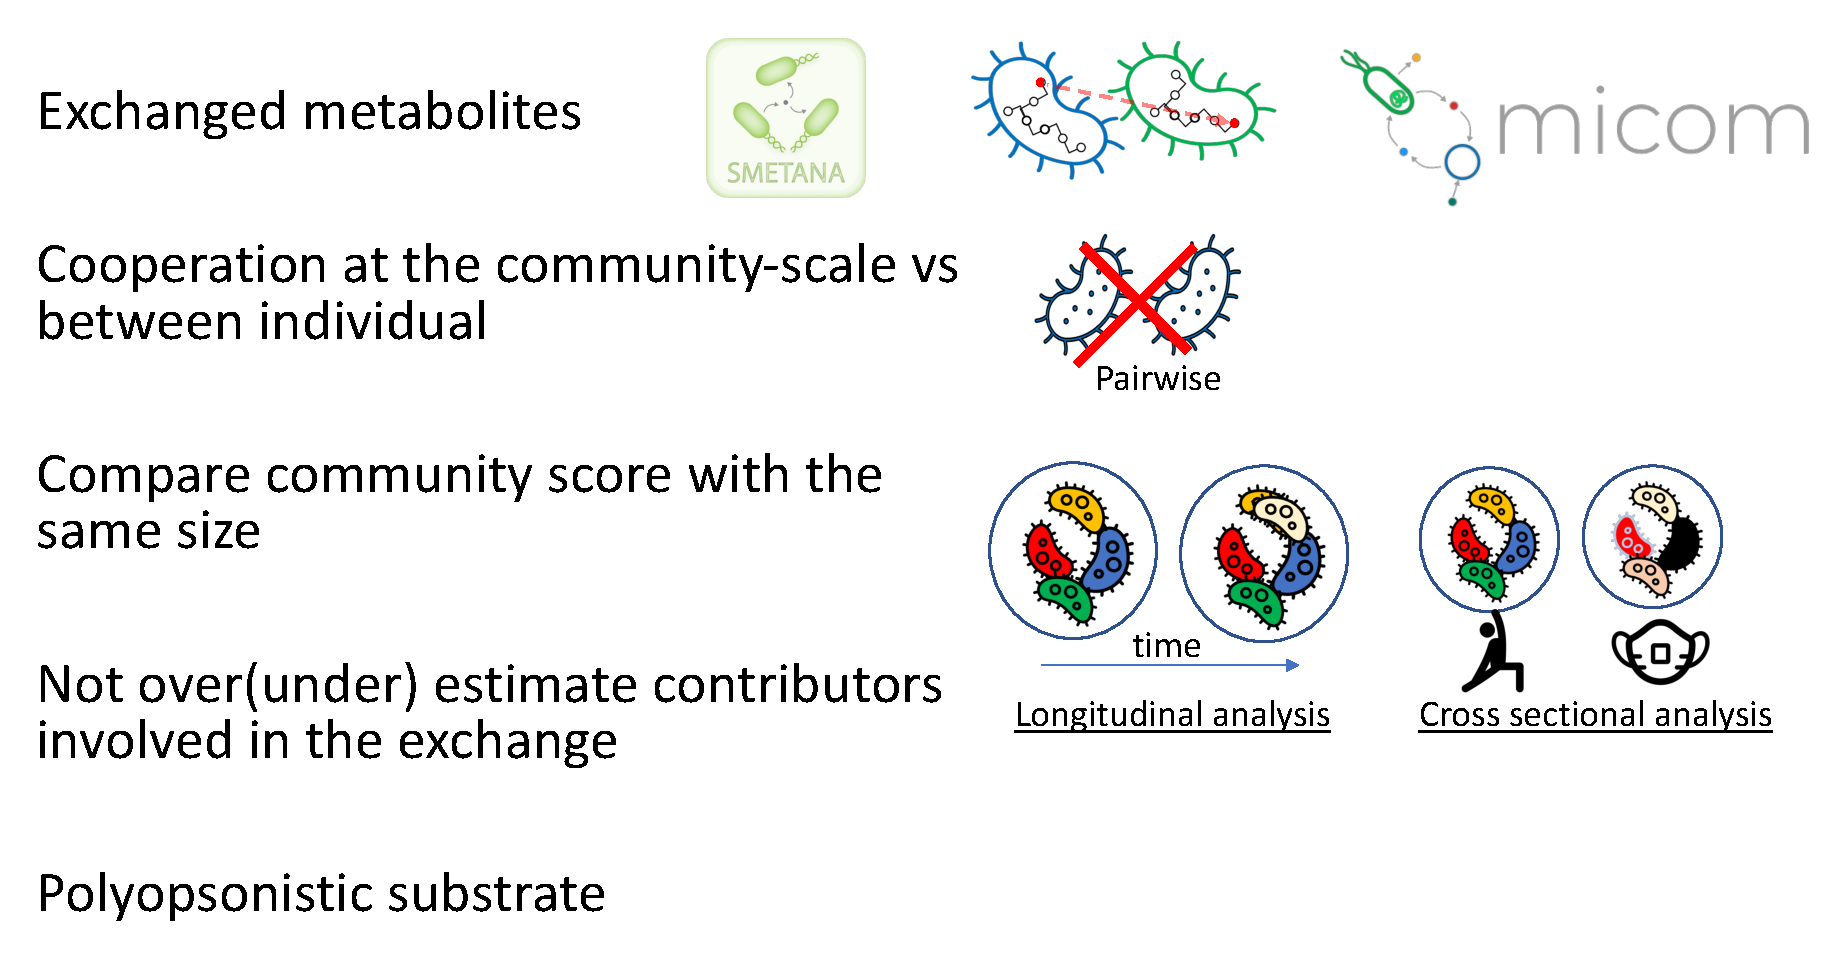
\includegraphics[width=\textwidth]{figures/coop-properties.pdf}
\begin{block}{}
\begin{itemize}
\item Inference of polyopsonistic substrate and exchanged compounds in logical rules (ASP)
\item Index of cooperation and competition in python
\end{itemize}
\end{block}
\end{frame}


\begin{frame}[fragile]
\frametitle{Potential interactions rules}
\begin{onlyenv}<1>
\framesubtitle{Cooperation rules development}
\begin{minipage}{0.5\textwidth}
\begin{lstlisting}[mathescape=True, label={lst:echange}] captionpos=b,style=aspwide]
exchange(M,P,C) :- taxon(P),
taxon(C),
P != C,
reactant(M,_,C),
product(M,_,P),
scope(metabolite(M,P), all),
not scope(metabolite(M,C), self(C)).
\end{lstlisting}
\begin{itemize}
	\item[ligne 1:] un métabolite \texttt{M} est échangeable entre un producteur \texttt{P} et un consommateur \texttt{C} si \texttt{P} est un taxon et 
	\item[ligne 2:] que \texttt{C} est un taxon et
	\item[ligne 3:] \texttt{P} est différent de \texttt{C} et
	\item[ligne 4:] que \texttt{M} est un réactant de n'importe quelle réaction de \texttt{C} et 
	\item[ligne 5:] que \texttt{M} est un produit de n'importe quelle réaction de \texttt{P} et
	\item[ligne 6:] que \texttt{M} est dans le \texttt{scope} communautaire produit par \texttt{P} et 
	\item[ligne 7:] que \texttt{M} n'est pas dans le \texttt{scope} de \texttt{C}.
\end{itemize}
\end{minipage}%
\hspace{0.25cm}
\hfill
\begin{minipage}{0.45\textwidth}
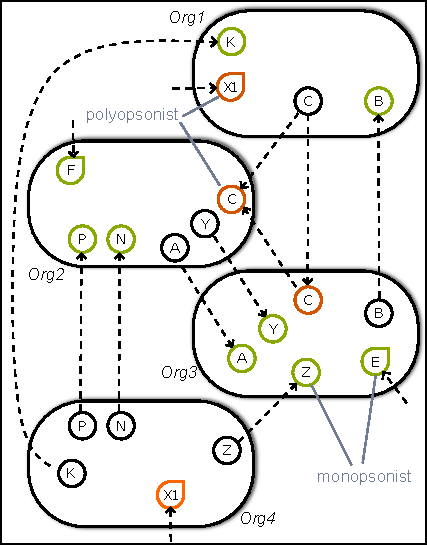
\includegraphics[width=\textwidth]{figures/poly-monoopsonie.pdf}
\end{minipage}

\end{onlyenv}

\begin{onlyenv}<2>
\framesubtitle{Competition rules}
\begin{minipage}{0.5\textwidth}
\begin{lstlisting}[mathescape=True,label={lst:competition}, captionpos=b]
% cas pour les metabolites echangeables
polyopsonist(M,N) :- N=#count{C,M:exchange(M,_,C)},
exchange(M,_,_), N > 1.
		 	
% cas pour les graines
polyopsonist(S,N) :- N=#count{B:seed_consumed_by_taxon(S,B)}, 
	N > 1, seed(S).
\end{lstlisting}
\begin{itemize}
	\item[ligne 2-3:] Un composé échangé \texttt{M} est limitant si lorsque le nombre de consommateurs \texttt{C} impliqués dans l'échange de ce métabolite \texttt{M} est strictement supérieur à 1.
	\item[ligne 6-7:] Une graine \texttt{M} est considérée limitante lorsque le nombre de consommateurs \texttt{C} de cette graine \texttt{M} est strictement supérieur à 1. \\
\end{itemize}
\end{minipage}%
\hspace{0.25cm}
\hfill
\begin{minipage}{0.45\textwidth}
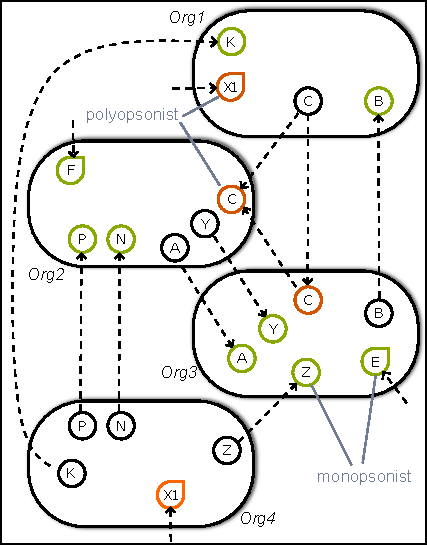
\includegraphics[width=\textwidth]{figures/poly-monoopsonie.pdf}
\end{minipage}
\end{onlyenv}
\end{frame}

\begin{frame}[fragile]
\frametitle{Scores}
\framesubtitle{Contributors}
\begin{onlyenv}<1>
\begin{minipage}{0.5\textwidth}
\vspace{-1cm}
\begin{block}{Goal}
Distinguish community with a difference in the number of consumers (resp. producers)
\end{block}
\textbf{Exchangeable metabolites}\\
2 --- C --- 2\\
1 --- A --- 1\\
1 --- B --- 1\\
1 --- Y --- 1

\[
w(k) = 2-{0.5^{k-1}}
\]

1.5 --- C --- 1.5\\
1 --- A --- 1\\
1 --- B --- 1\\
1 --- Y --- 1

\[
\begin{split}
    \textsf{CooP} &= \sum_{m\in M} w(|P_m|) + \sum_{m\in M} w(|C_m|)\\
     \textsf{CooP} &=  9
\end{split}
\]


\end{minipage}%
\hspace{0.5cm}
\hfill
\begin{minipage}{0.4\textwidth}
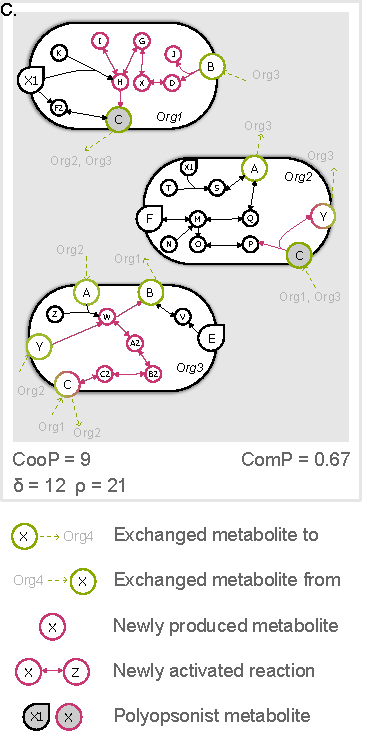
\includegraphics[width=\textwidth]{figures/score-taille-3.pdf}
\end{minipage}
\end{onlyenv}



\begin{onlyenv}<2>
\framesubtitle{Polyopsonistic, $\rho$ and $\delta$}
\begin{minipage}{0.5\textwidth}
\vspace{-1cm}
\begin{exampleblock}{Polyopsonistic}
Number of consumers involve in exchangeable metabolites and seed > 1
\end{exampleblock}{}

C --- 2

\begin{lstlisting}[mathescape=True]
 Comp = sum(polyopsonist.values())) / len(community.taxa)
 Comp = 0.67
\end{lstlisting}

\begin{exampleblock}{$\rho$}
Identify the reactionary added-value between the reaction scope in community and individually
\end{exampleblock}{}

\begin{exampleblock}{$\delta$}
Identify the producible compounds added-value between the metabolite scope in community and individually
\end{exampleblock}{}

\end{minipage}%
\hspace{0.5cm}
\hfill
\begin{minipage}{0.4\textwidth}
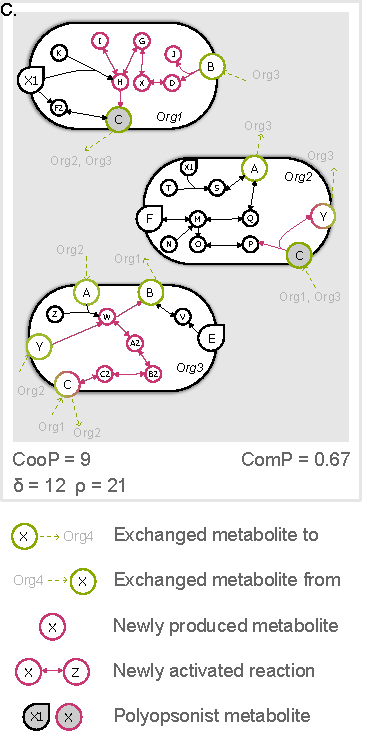
\includegraphics[width=\textwidth]{figures/score-taille-3.pdf}
\end{minipage}
\end{onlyenv}



\end{frame}

\tiny
\printbibliography


\end{document}
